\documentclass{beamer}

\mode<presentation> {
\usetheme{Madrid}
}

\usepackage[]{algorithm2e}
\usepackage{graphicx} 
\usepackage{booktabs} 

\graphicspath{{./images/}}


\title[HRL]{Regularized Hierarchical Policies for Compositional Transfer in Robotics} 

\author{Sreejith Krishnan R}
\institute[CET]
{
College Of Engineering, Trivandrum \\ 
\medskip
\textit{Robotics \& Automation}
}
\date{\today} 

\begin{document}

\begin{frame}
\titlepage 
\end{frame}

\section{Introduction} 

\subsection{Reinforcement Learning} 

\begin{frame}
\frametitle{Reinforcement Learning}
\begin{center}
	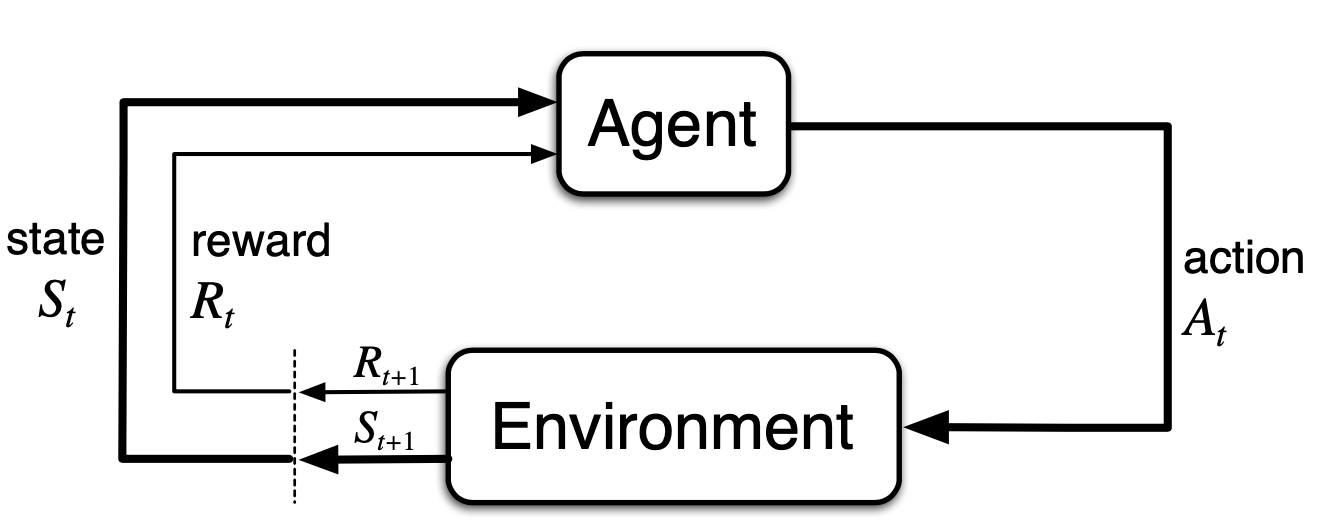
\includegraphics[scale=0.3]{mdp.png}
\end{center}

\begin{itemize}
	\item Agent interacts with the environment at state $s_t \epsilon S$ by taking action $a_t \epsilon A$ according to policy $\pi(a_t|s_t)$
	\item Upon action from agent, environment state will transition to state $s_{t+1}$ according to transition dynamics $p(s_{t+1}|s_t,a_t)$ and return a reward $r_t \epsilon R$
	\item Objective of reinforcement learning is to find the policy $\pi(a_t|s_t)$ so as to maximize the expected reward $V^{\pi}(s_0) = E_{\pi} [\sum_{t=0}^{\infty} \gamma^t r(s_t, a_t)]$
\end{itemize}
\end{frame}

%------------------------------------------------

\begin{frame}
\frametitle{Value based RL}
\begin{columns}[c]
	
	\column{.5\textwidth}
	\begin{itemize}
		\item Policy $\pi^{\theta}(s_t, a_t) = Q(s_t, a_t; \theta)$ predicts the expected reward of choosing $a_t$ at state $s_t$
		\item Agent select action $a_t$ with maximum expected reward
		\item After taking action $a_t$, environment transitions to $s_{t+1}$ and gives reward $r_t$
	\end{itemize}
	
	\column{.5\textwidth}
	\begin{center}
		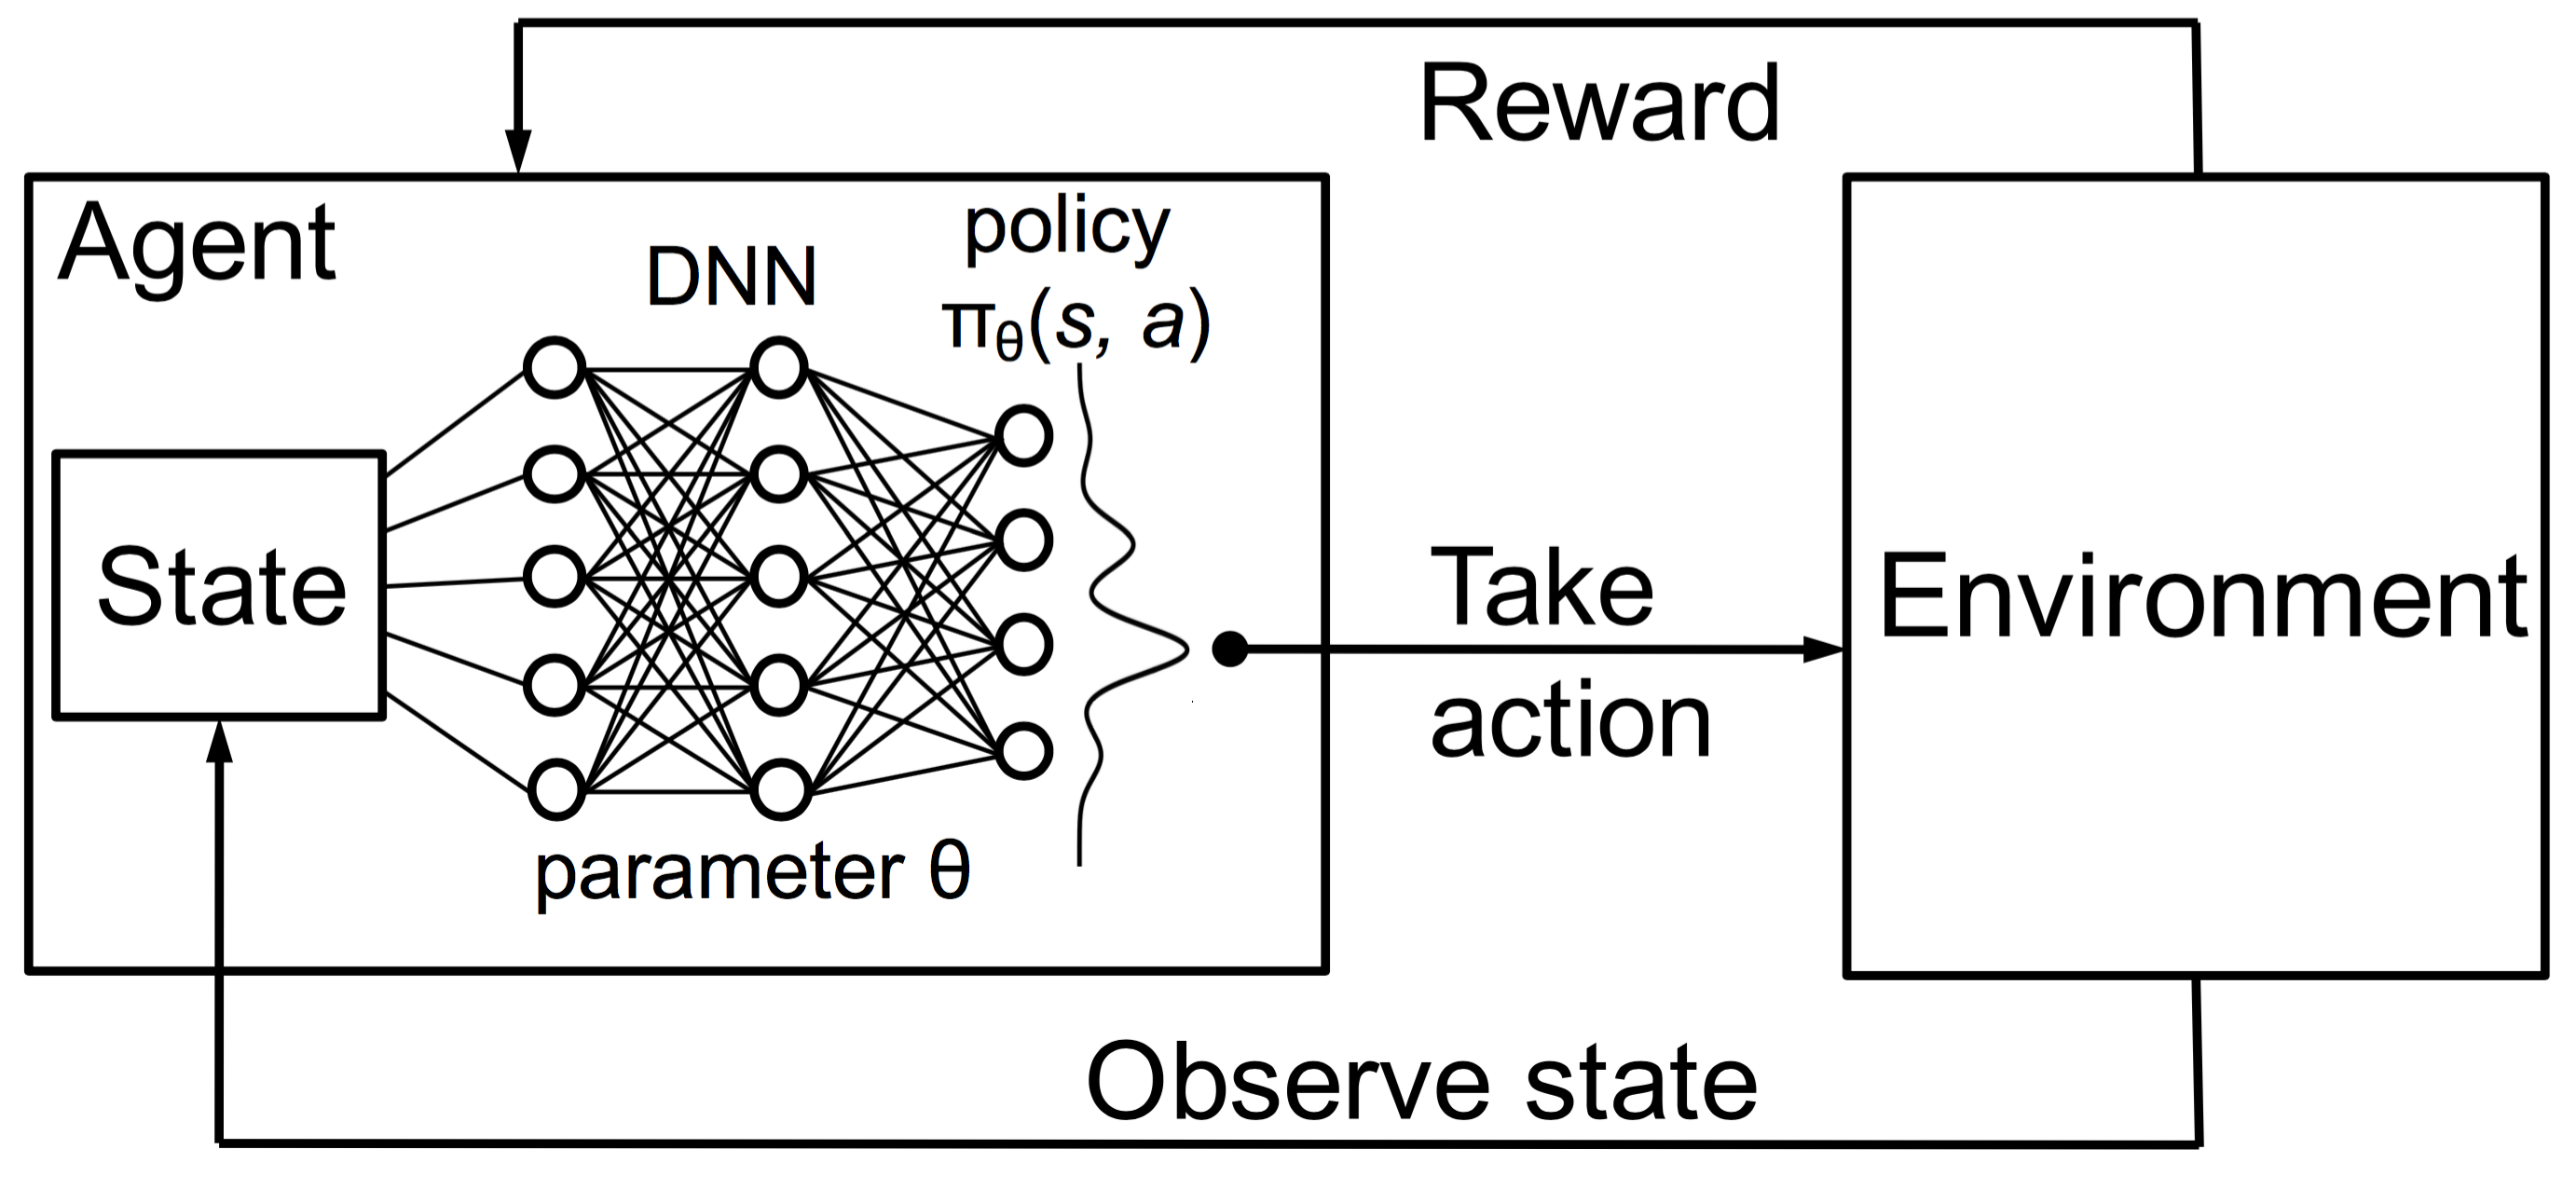
\includegraphics[scale=0.06]{dqn.png}
	\end{center}
	
\end{columns}

\begin{itemize}
	\item Parameters $\theta$ of policy $\pi^{\theta}(s_t, a_t)$ is adjusted to minimize the loss function $L(\theta) = (\hat{Q}(s_t, a_t) - Q(s_t, a_t; \theta))^2$
\end{itemize}

\end{frame}

%------------------------------------------------

\begin{frame}
\frametitle{Policy based RL}
\begin{itemize}
	\item Policy based RL methods directly output the probability of taking an action instead of estimating the Q value
	\item Can be used for both continuous and discrete action space
	\item For continuous action space, mean and variance of a normal distribution is estimated and action is sampled from this distribution
	\item Common algorithms :- Policy Gradients and PPO
\end{itemize}
\end{frame}

\begin{frame}
\frametitle{Regularized Hierarchical Policies}
	\textbf{Policy}
	\begin{equation}
	\pi_{\theta} (a | s, i) = \sum_{O=1}^{M} \pi_{\theta}^L(a | s, o) \pi_{\theta}^H(o | s, i)
	\end{equation}
	
	\textbf{Objective}
	\begin{equation}
	\underset{q}{max} J(q, \pi_{ref}) = E_{i \sim I} \left[ E_{\pi, s \sim D} \left[ \sum_{t=0}^{\infty} \gamma^t r_i(s_t, a_t) | s_{t+1} \sim p(.|_t, a_t) \right] \right]
	\end{equation}
	subject to constraint
	\begin{equation}
		E_{s \sim D, i \sim I} \left[ KL(q(. | s, i) || \pi_{ref}(. | s, i)) \right] \leq \epsilon
	\end{equation}
\end{frame}

\begin{frame}
	\frametitle{Regularized Hierarchical Policies}
	\framesubtitle{Algorithm - Learner}
	
	\begin{center}
		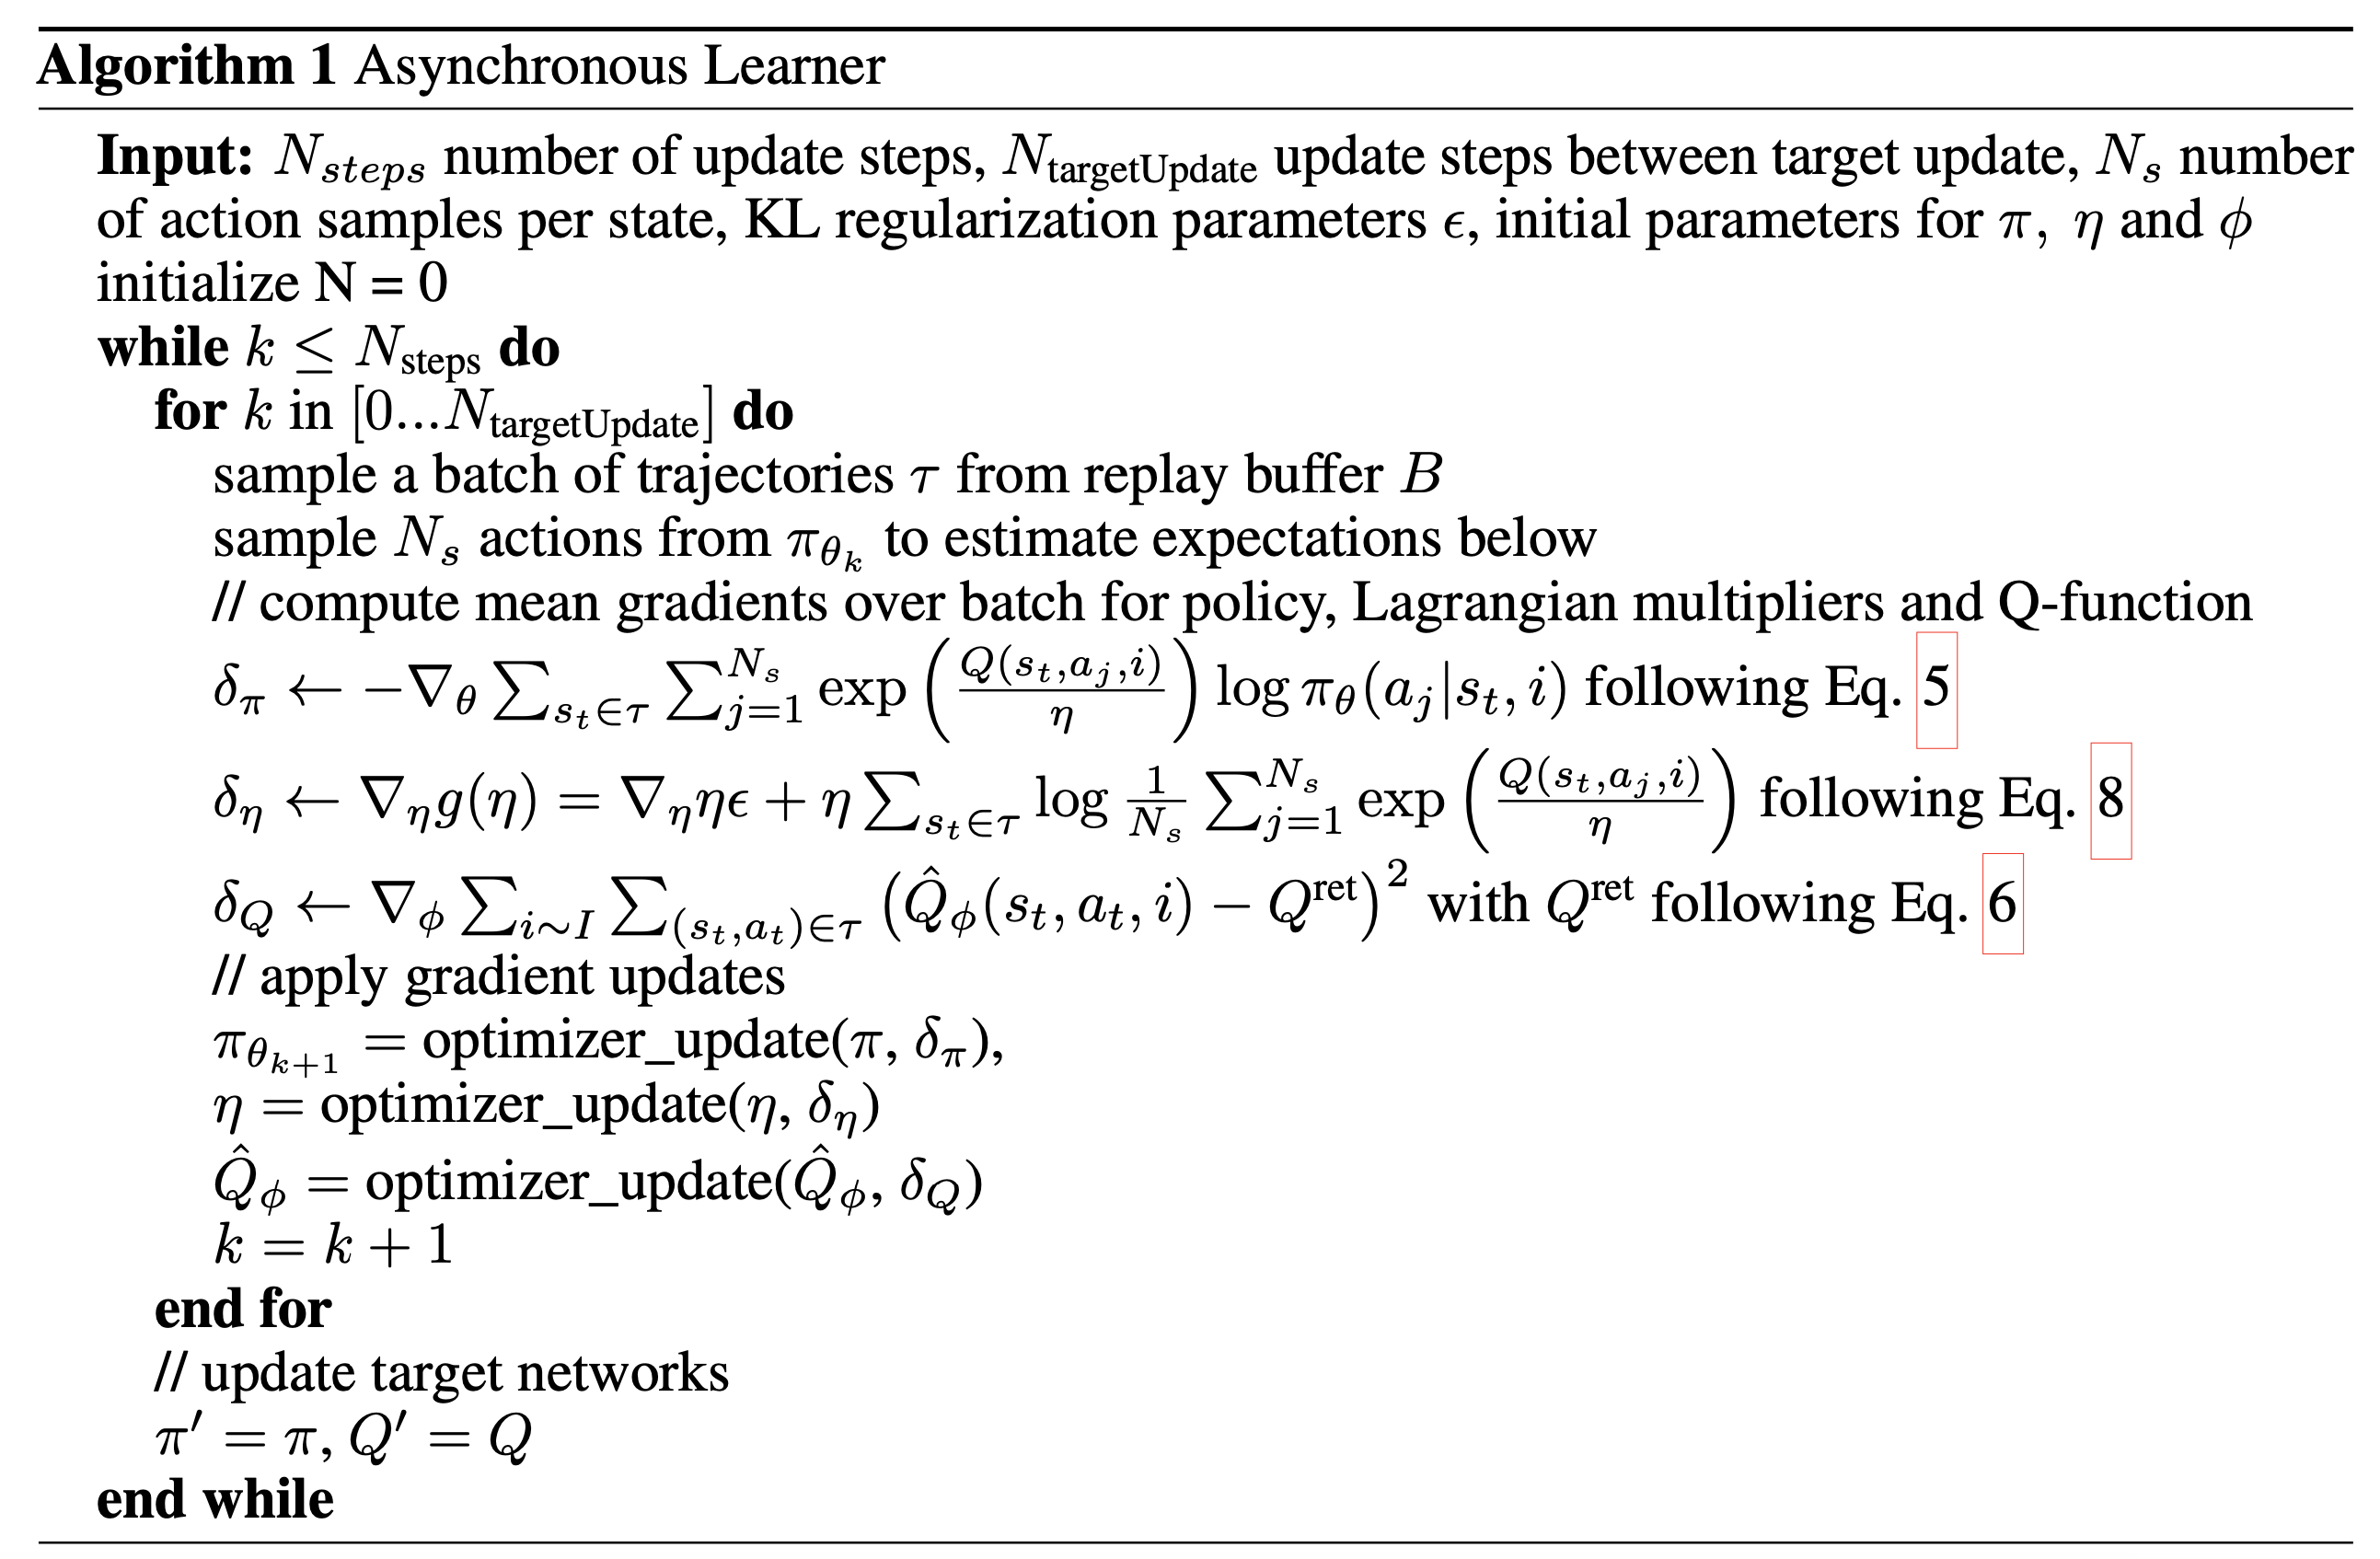
\includegraphics[scale=0.25]{algorithm-learner}
	\end{center}
	
\end{frame}

\begin{frame}
	\frametitle{Regularized Hierarchical Policies}
	\framesubtitle{Algorithm - Actor}
	
	\begin{center}
		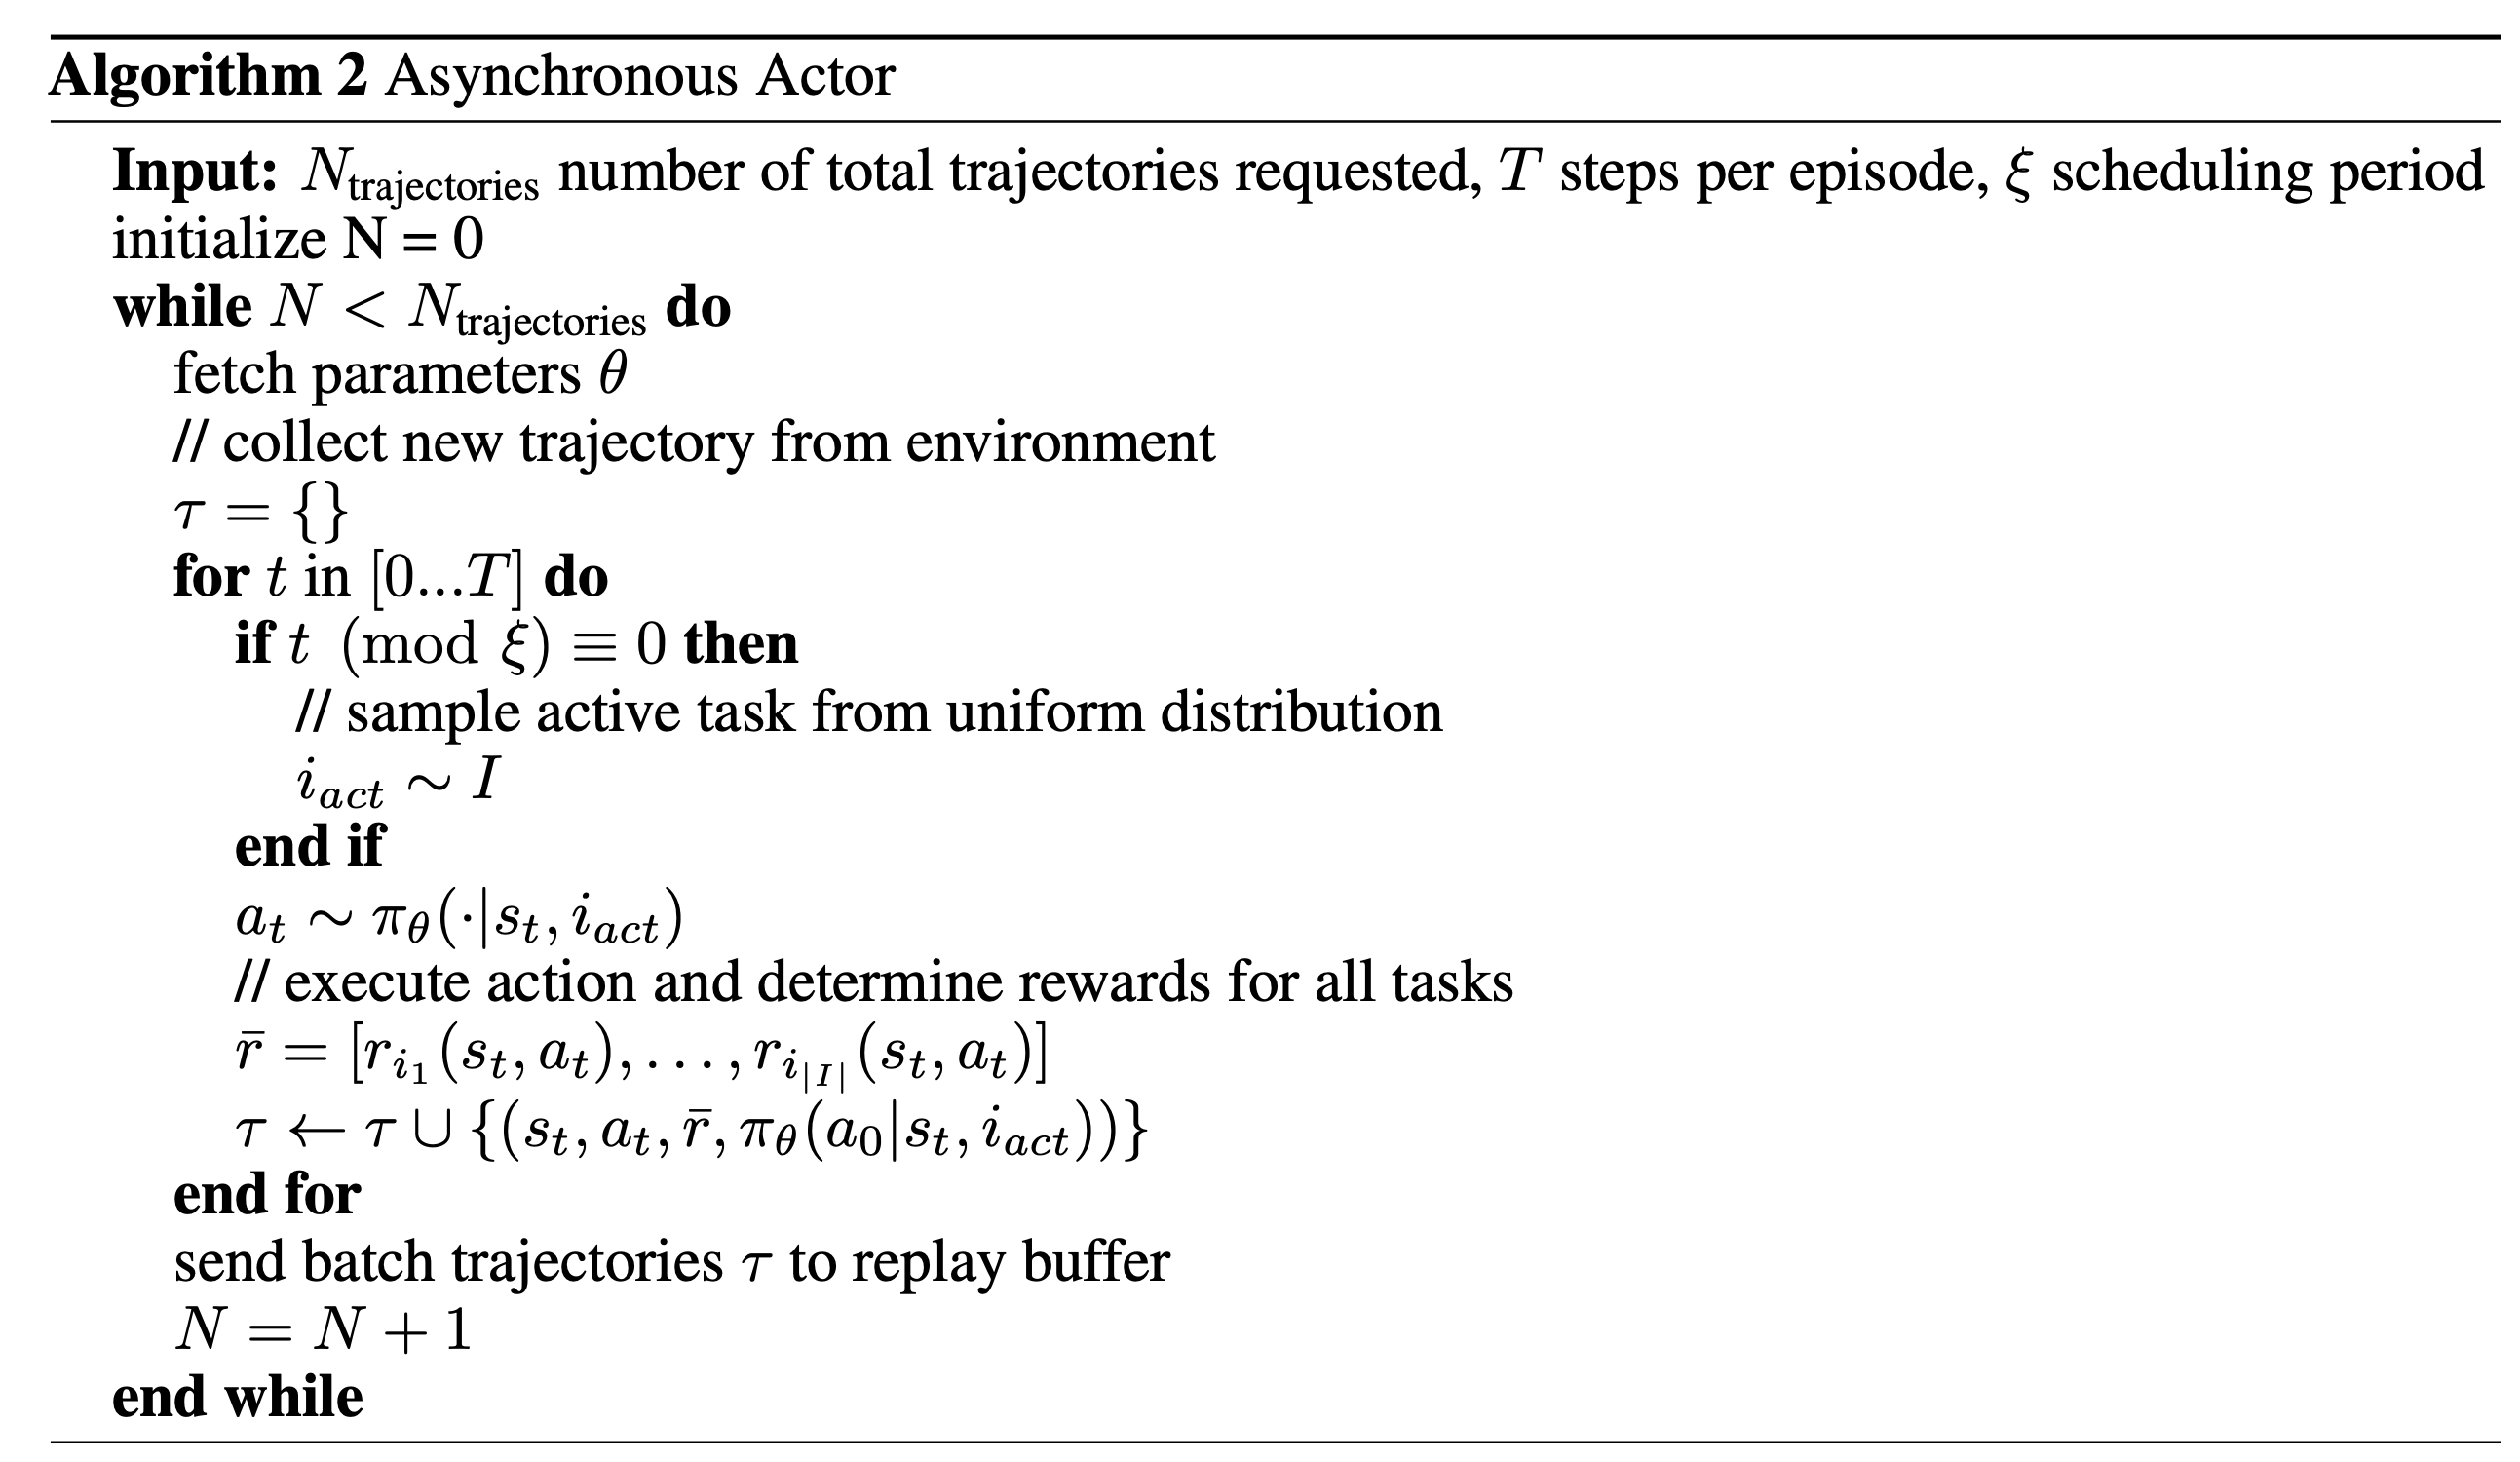
\includegraphics[scale=0.25]{algorithm-actor}
	\end{center}
	
\end{frame}

%------------------------------------------------

\begin{frame}
	\frametitle{Regularized Hierarchical Policies}
	\framesubtitle{Architecture}
	
	\begin{columns}
		\column{0.5\textwidth}
		\centering{RHPO architecture}
		
		\column{0.5\textwidth}
		\centering{Monolithic architecture}
	\end{columns}

	\begin{columns}
		\column{0.5\textwidth}
		\begin{figure}[H]
			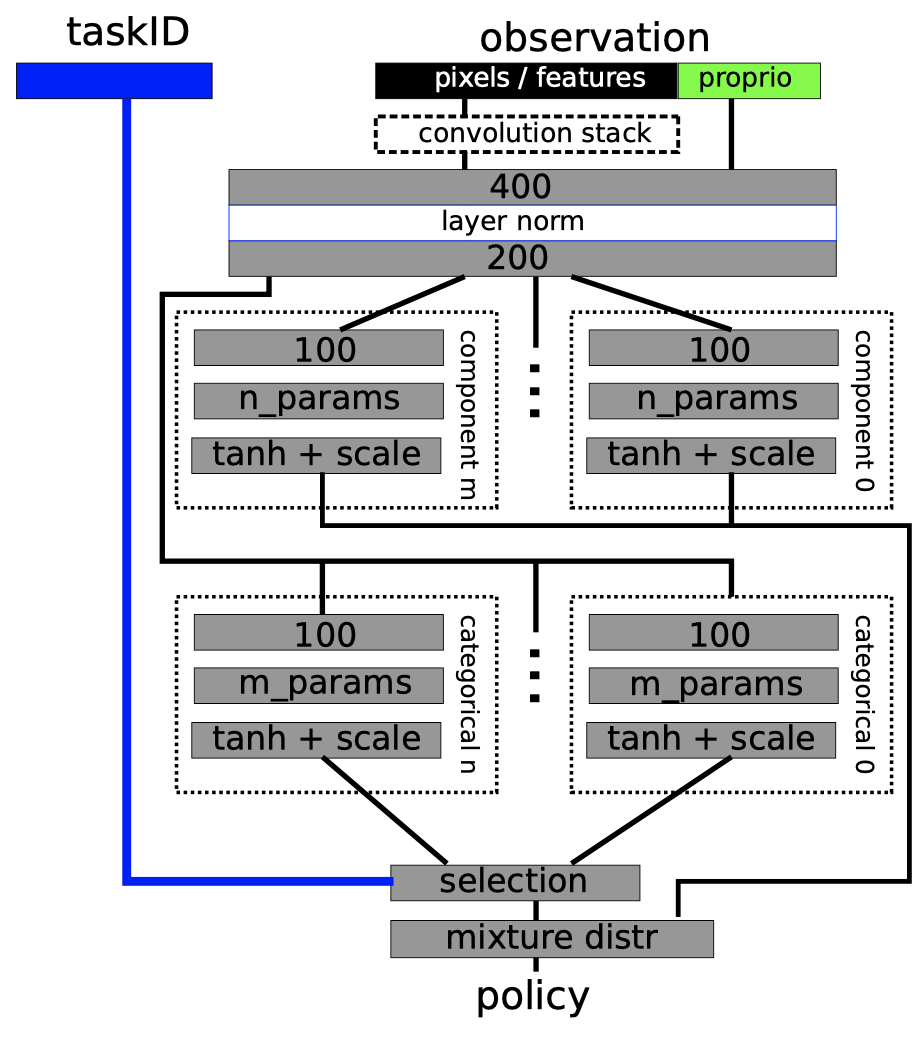
\includegraphics[scale=0.3]{rhpo-arch.png}
		\end{figure}
	
		\column{0.5\textwidth}
		\begin{figure}[H]
			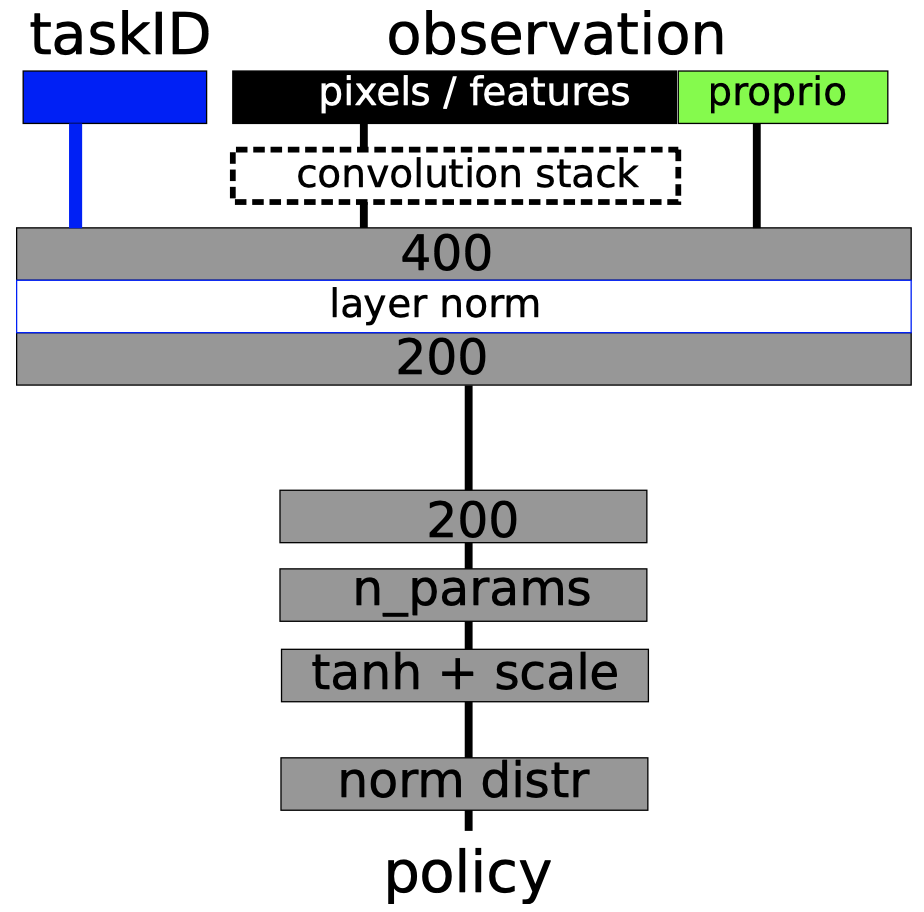
\includegraphics[scale=0.3]{monolithic-arch.png}
		\end{figure}
	\end{columns}
\end{frame}

\begin{frame}
	\frametitle{Experiments}
	\framesubtitle{Exp 1 - Simulation - Setup}
	
	\begin{columns}[c]
		
		\column{.5\textwidth}

		\begin{itemize}
			\item 7DOF robot arm with parallel gripper
			\item Environment consists 3 cubes of colour yellow, blue and green with edge length 5cm
			\item Task is to place green cube over yellow cube
		\end{itemize}
		
		\column{.45\textwidth}
		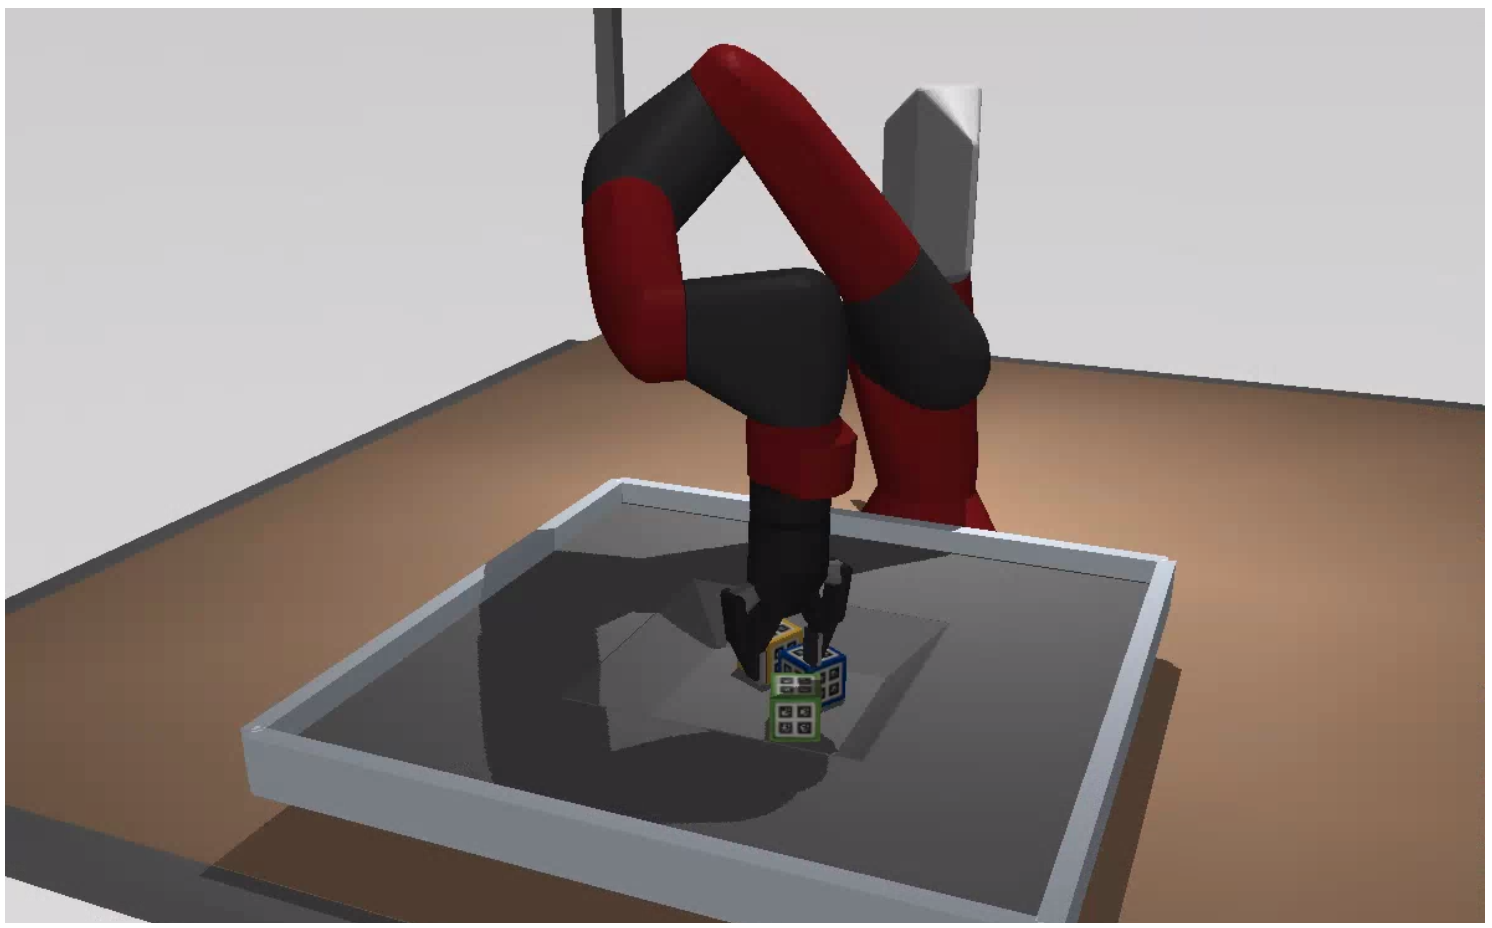
\includegraphics[scale=0.2]{sim1.png}
		
	\end{columns}

	\begin{itemize}
		\item Sub tasks are REACH(G), GRASP(G), LIFT(G), PLACE\_WIDE(G,Y), PLACE\_NARROW(G,Y), STACK(G,Y)  and LEAVE(G,Y)
		\item Action space is $\{v_x, v_y, v_z, wrist_{\omega}, v_{finger}\}$
		\item Inputs are joint positions, velocities and torques, tool centre position, gripper motor position and velocity, binary grasp flag, wrist sensor force and torque readings and cube poses
	\end{itemize}
\end{frame}

\begin{frame}
	\frametitle{Experiments}
	\framesubtitle{Exp 1 - Real robot  - Setup}
	
	\begin{columns}[c]
		
		\column{.5\textwidth}
		
		\begin{itemize}
			\item Sawyer robot arm mounted on a table and equipped with a Robotiq 2F-85 parallel gripper.
			\item Three cameras on the basket track cubes to estimate their pose using Augmented Reality tags
		\end{itemize}
		
		\column{.45\textwidth}
		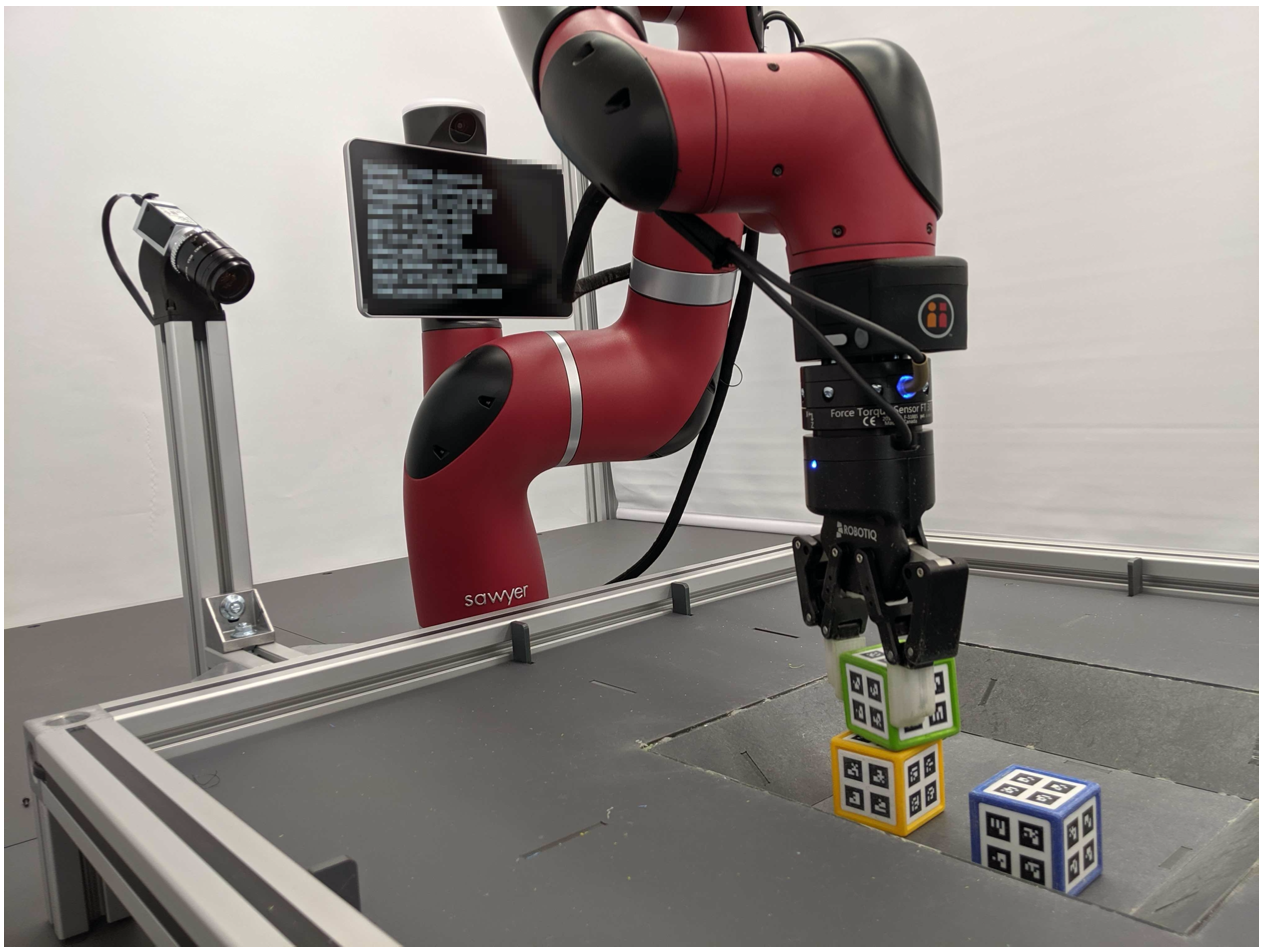
\includegraphics[scale=0.2]{exp1.png}
		
	\end{columns}
	
	\begin{itemize}
		\item Environment setup, action space and inputs are same as simulation
	\end{itemize}
\end{frame}

\begin{frame}
	\frametitle{Experiments}
	\framesubtitle{Exp 1 - Results}
	
	\begin{columns}[c]
		\column{.5\textwidth} 
		\begin{figure}[h!]
			\caption{Real robot: Reach}
			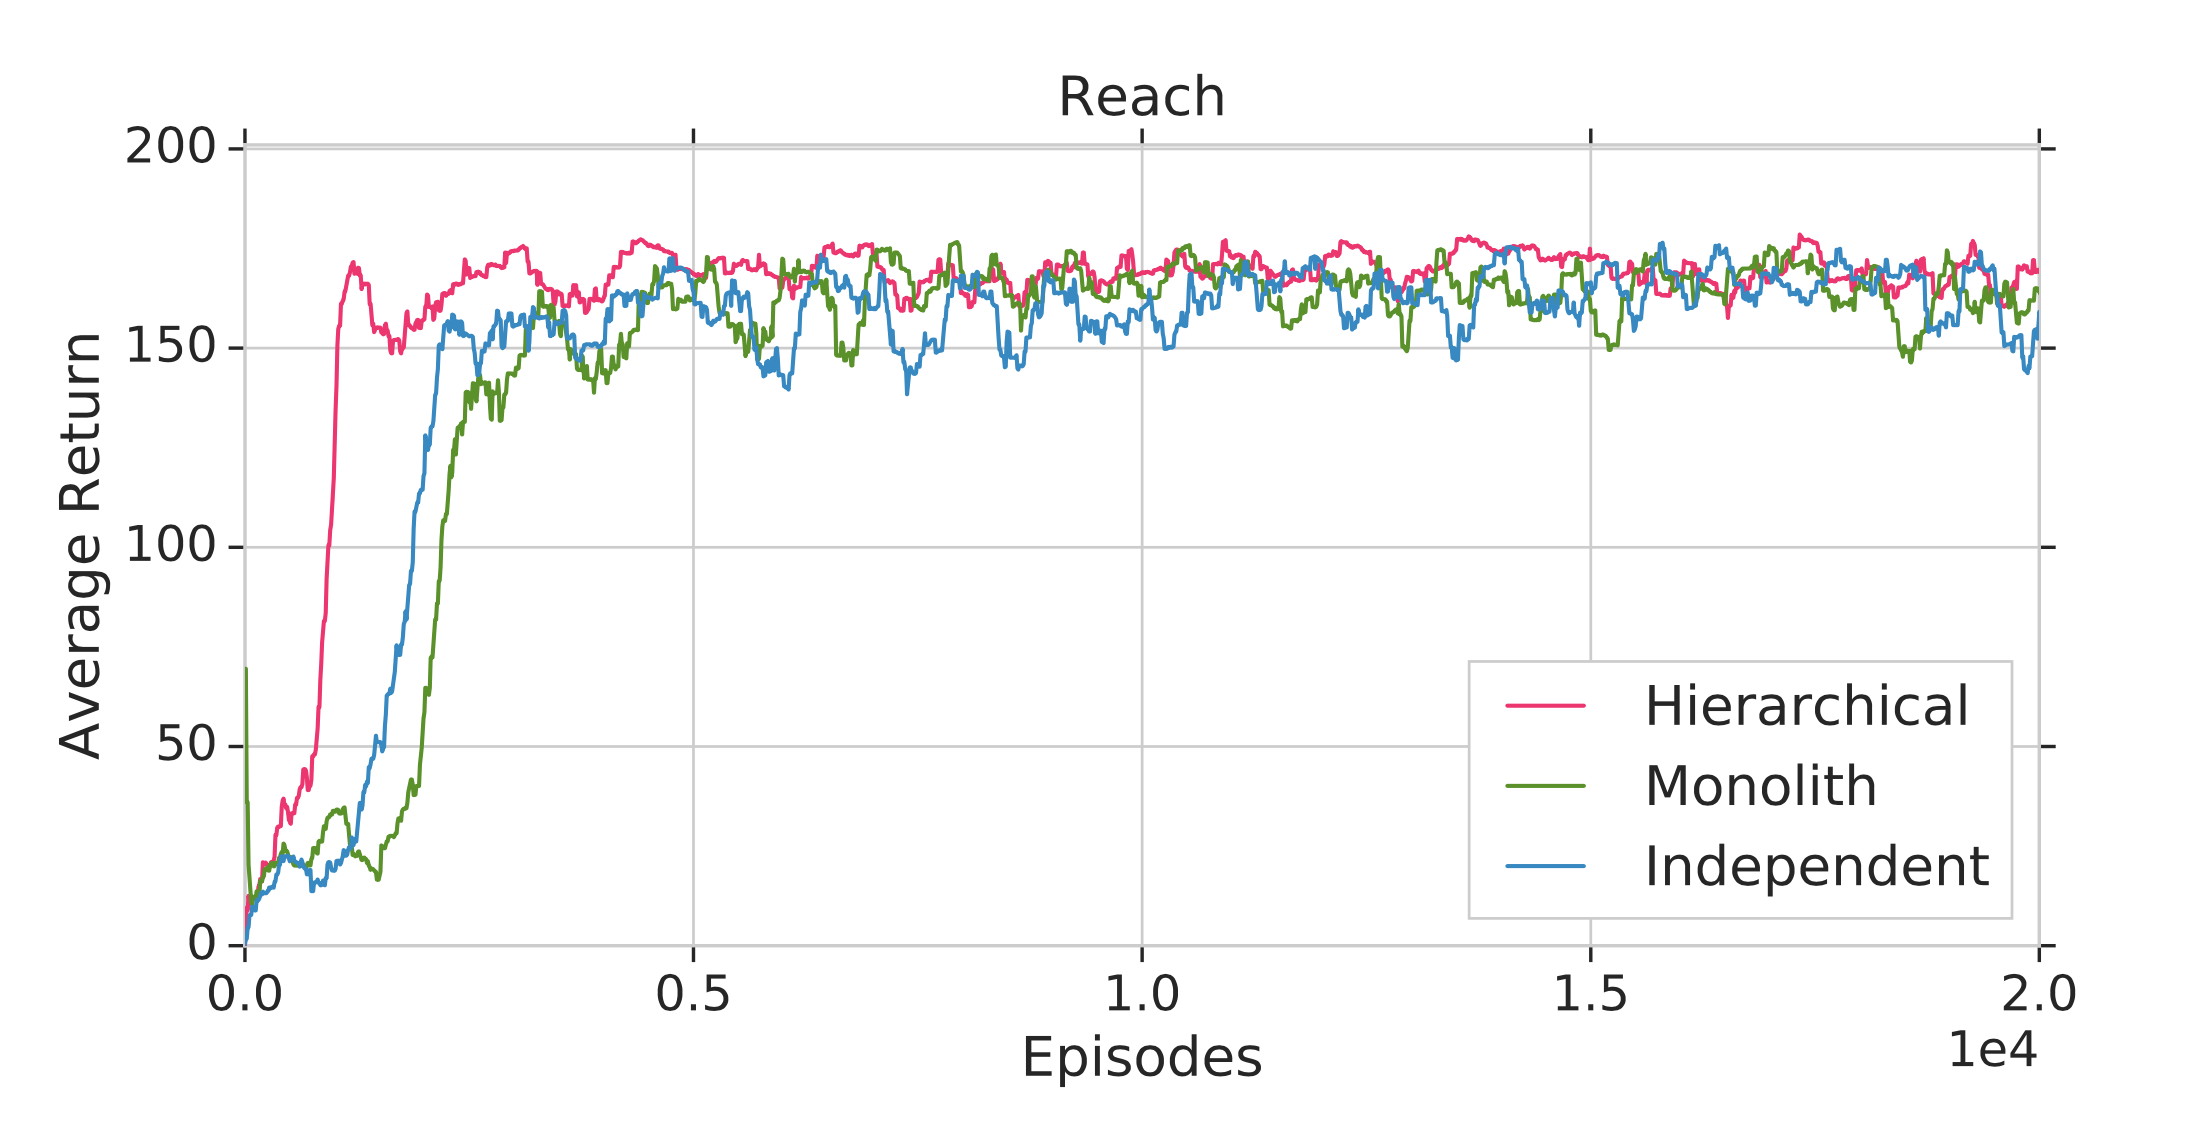
\includegraphics[scale=0.12]{exp-r1-1.png}
		\end{figure}
		
		\column{.5\textwidth}
		\begin{figure}[h!]
			\caption{Real robot: Stack}
			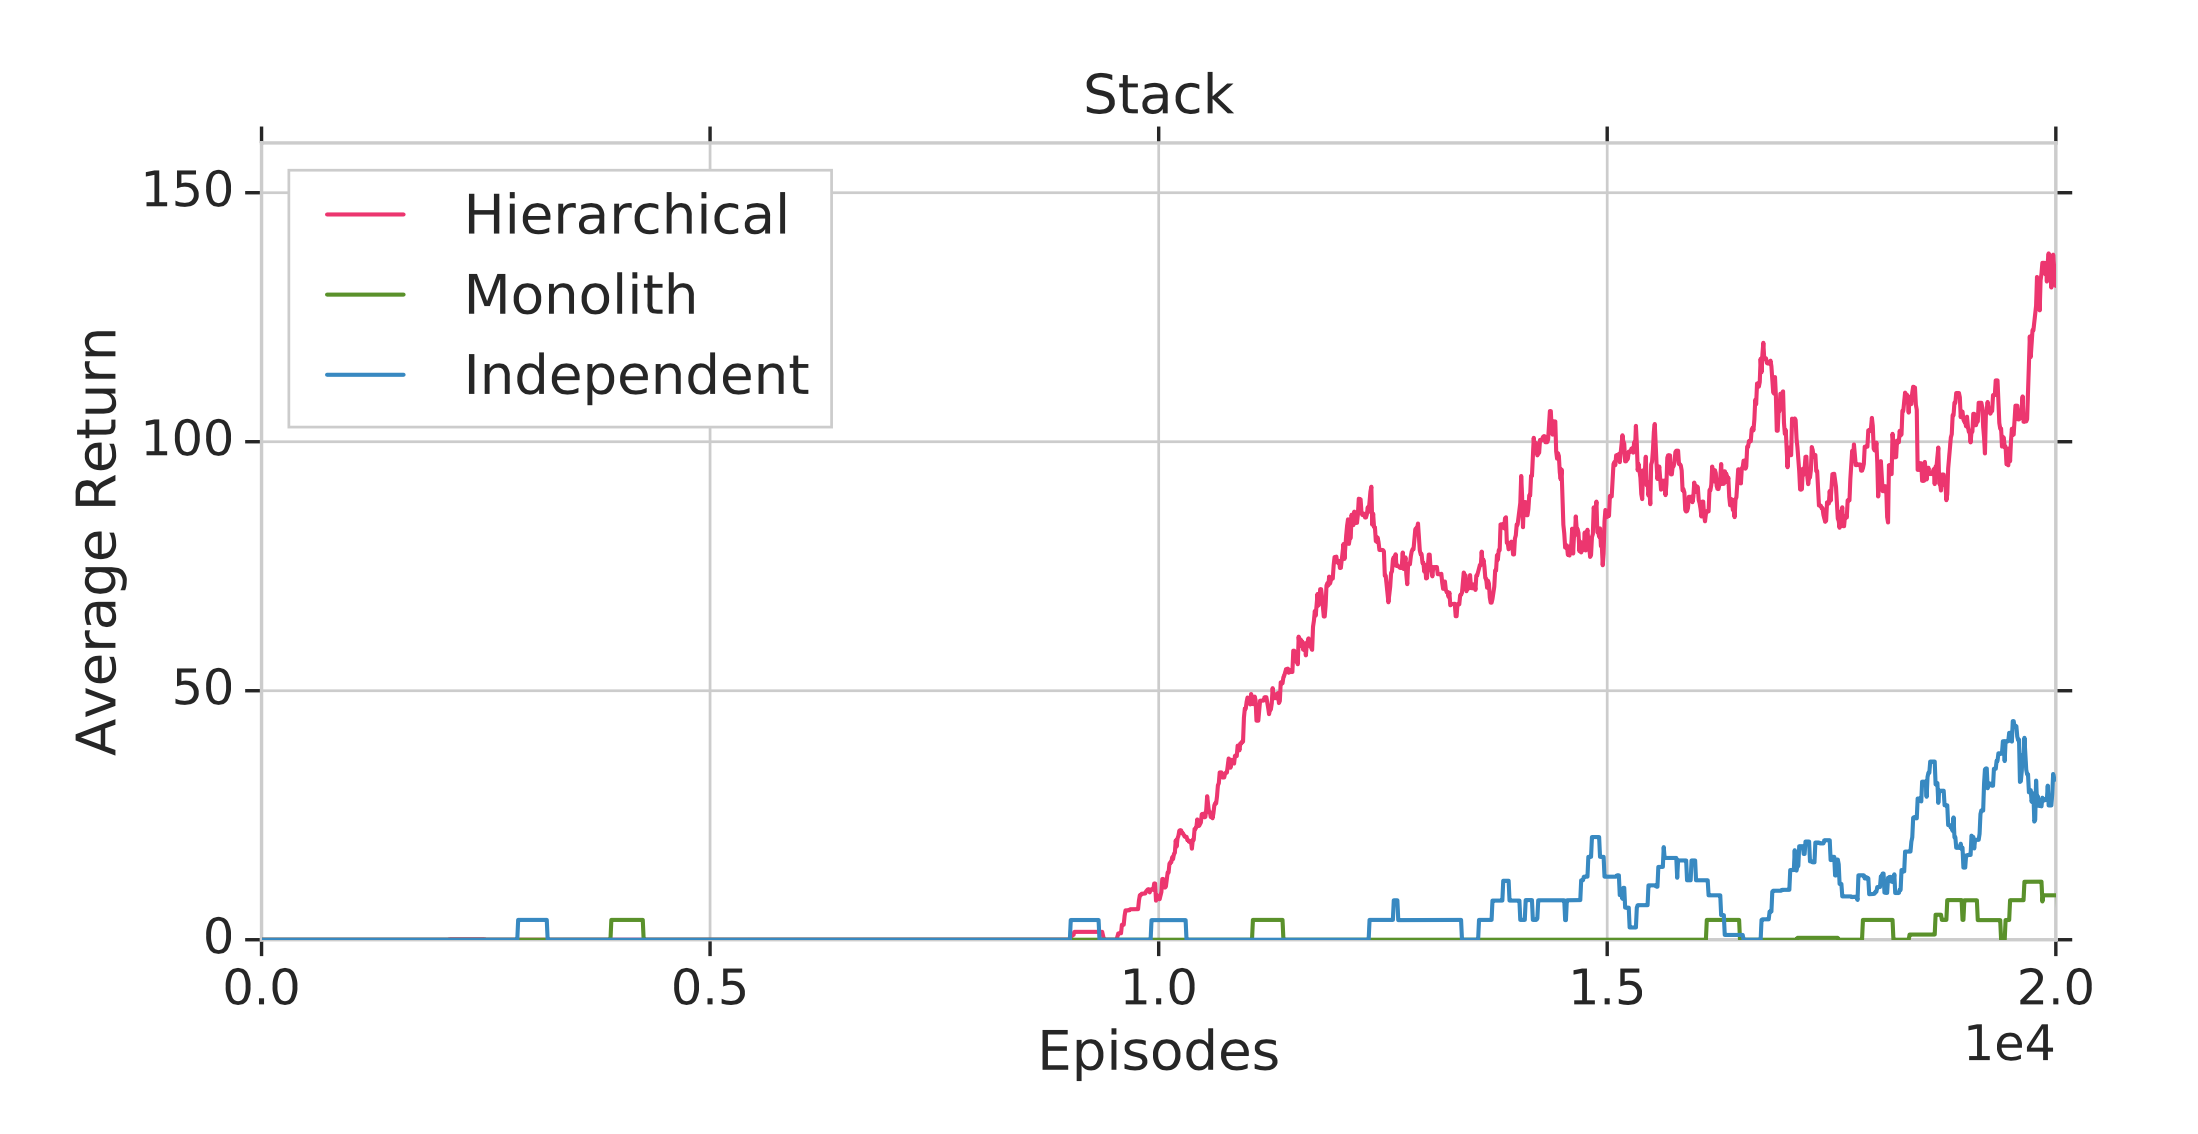
\includegraphics[scale=0.12]{exp-r1-2.png}
		\end{figure}
	\end{columns}
	
	\begin{figure}[h!]
		\caption{Simulation: Reach, Stack and Leave}
		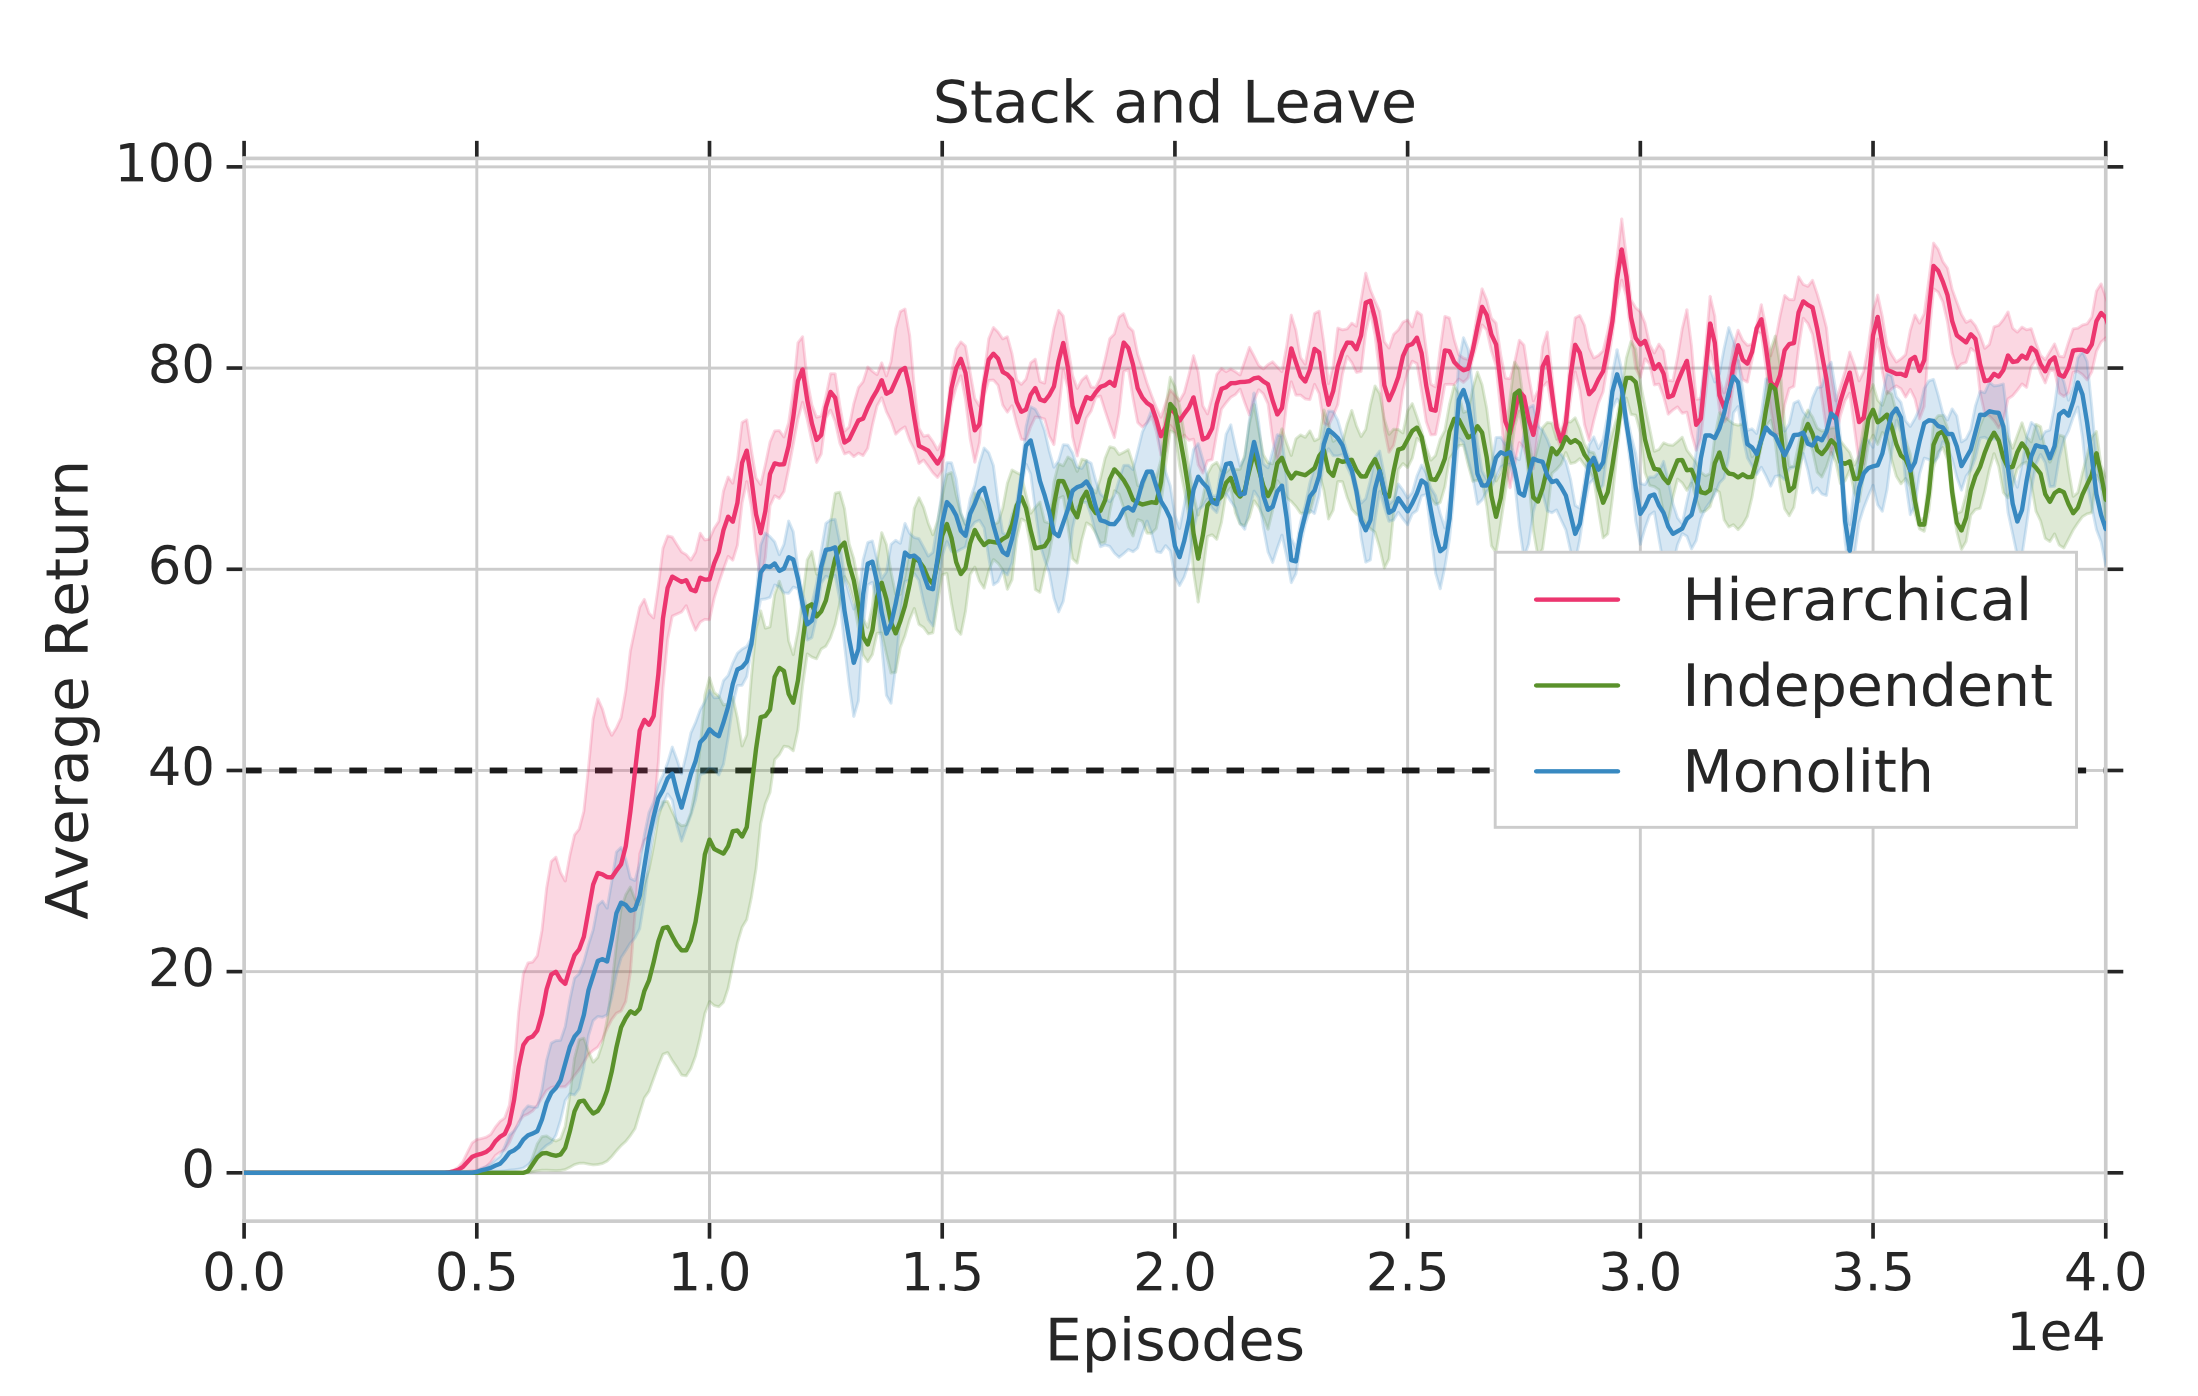
\includegraphics[scale=0.12]{sim-r1.png}
	\end{figure}
\end{frame}

\begin{frame}
	\frametitle{Experiments}
	\framesubtitle{Exp 2 - Simulation - Setup}
	
	\begin{columns}[c]
		
		\column{.5\textwidth}
		
		\begin{itemize}
			\item Kinova Jaco robot arm, equipped with a Kinova KG-3 gripper
			\item Environment consists 2 cubes of colour red and blue with edge length 5cm
			\item Task is to place blue cube over red cube and then place red over blue cube
		\end{itemize}
		
		\column{.45\textwidth}
		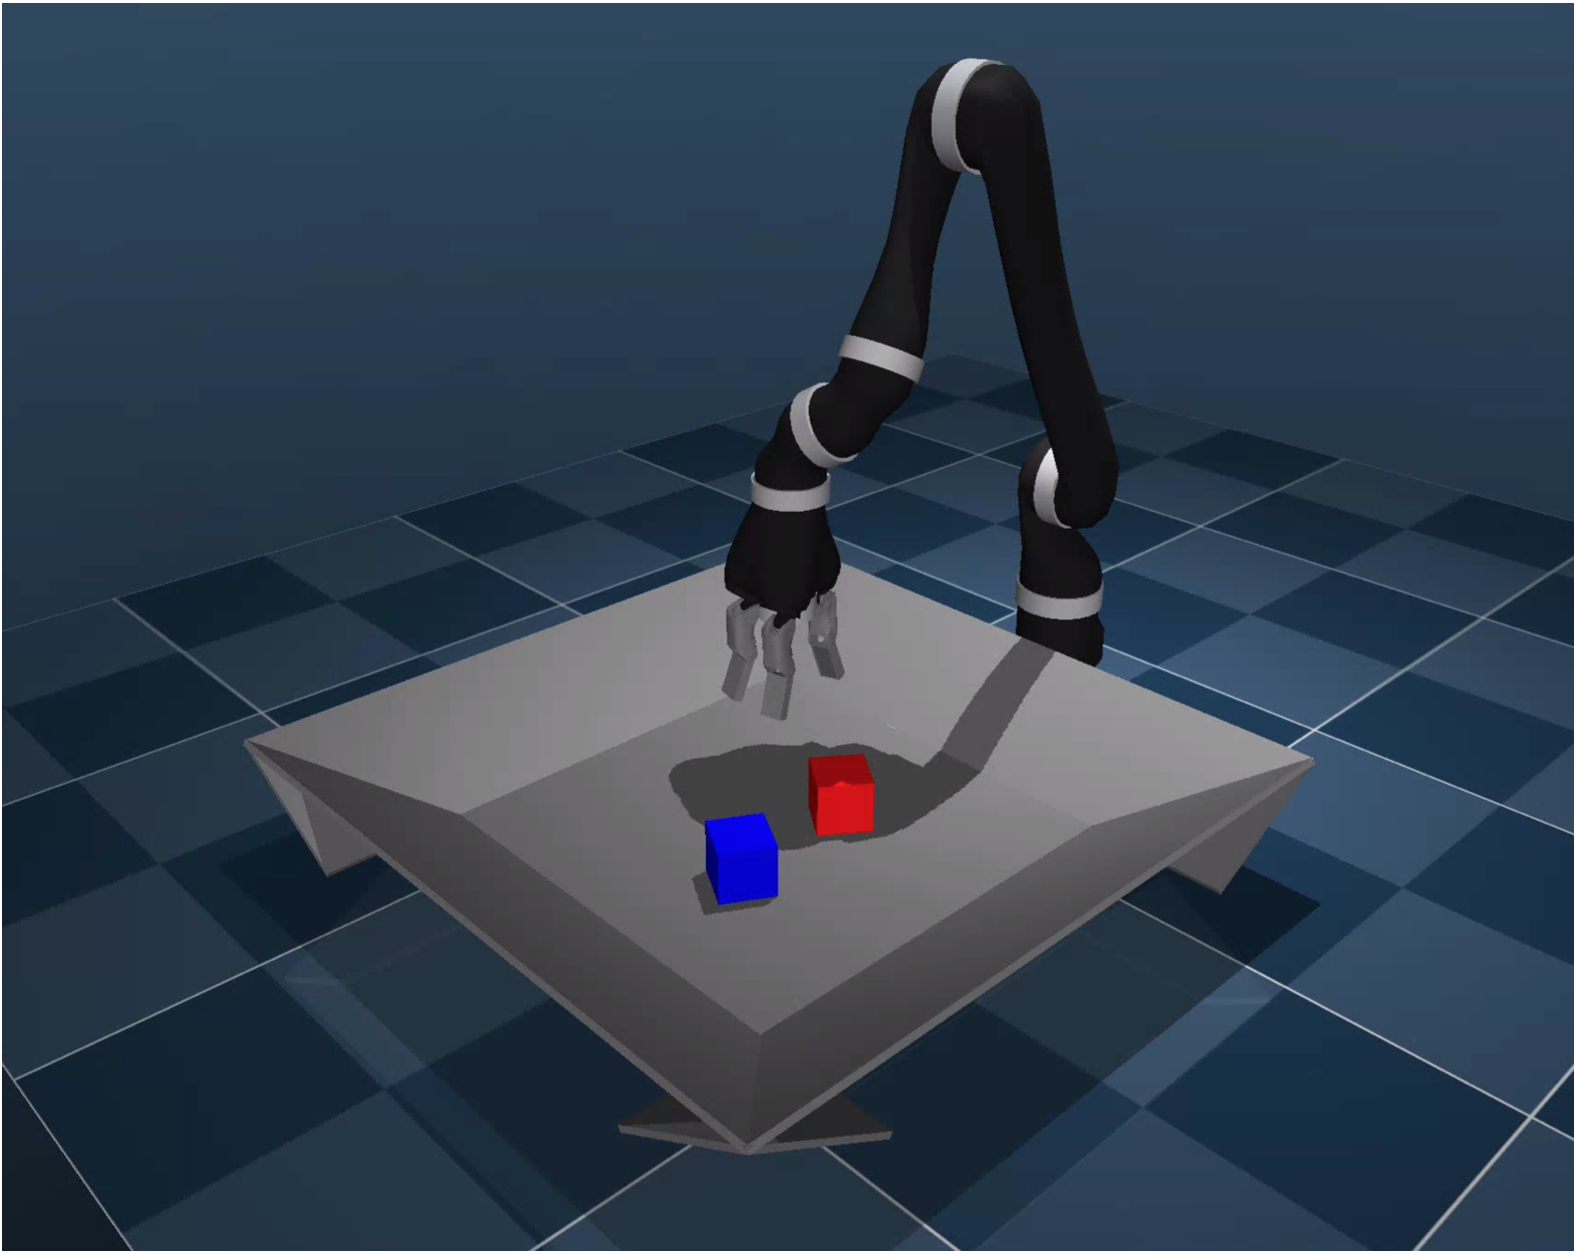
\includegraphics[scale=0.2]{sim2.png}
		
	\end{columns}
	
	\begin{itemize}
		\item Action space is
		\begin{center}
			\begin{tabular}{cccc}
				\hline 
				Entry & Dimension & Unit & Range \\ 
				\hline 
				Joint velocity (Arm) & 6 & rad/s & [-0.8,0.8] \\ 
				\hline 
				Joint velocity (Hand) & 3 & rad/s & [-0.8,0.8] \\ 
				\hline 
			\end{tabular} 
		\end{center}
		\item Inputs are same as exp 1
	\end{itemize}
\end{frame}

\begin{frame}
	\frametitle{Experiments}
	\framesubtitle{Exp 2 - Results}
	
	\begin{figure}[!h]
		\caption{Simulation: Exp 2}
		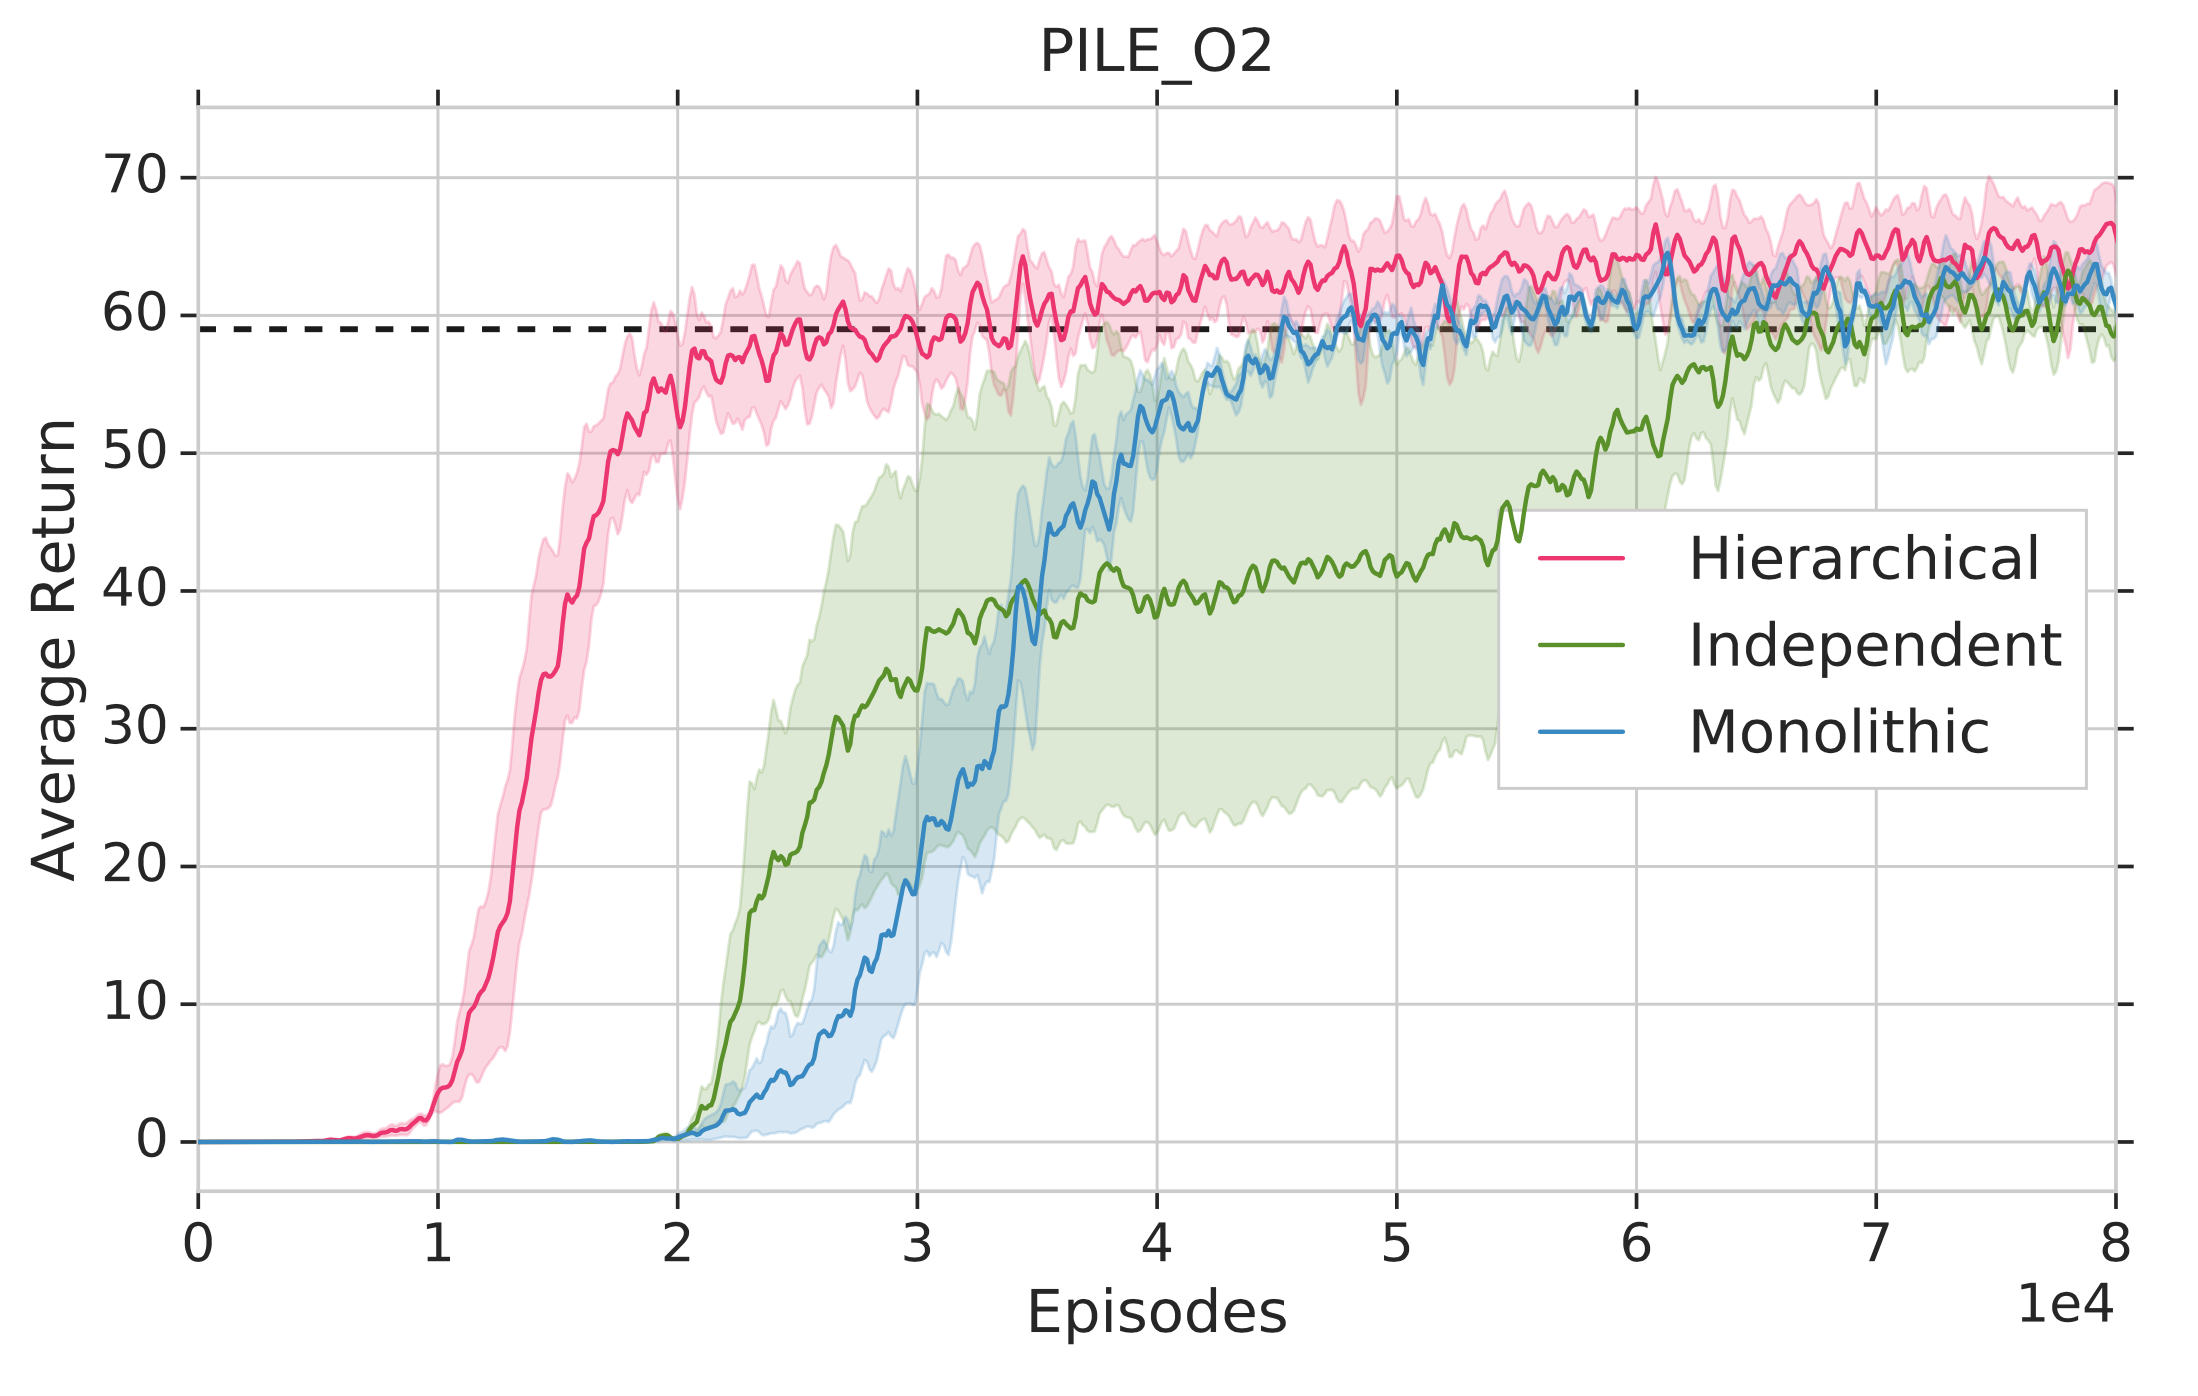
\includegraphics[scale=0.2]{sim-r2.png}
	\end{figure}
\end{frame}

\begin{frame}
	\frametitle{Experiments}
	\framesubtitle{Exp 3 - Simulation - Setup}
	
	\begin{columns}[c]
		
		\column{.5\textwidth}
		
		\begin{itemize}
			\item Same robot setup as exp 2
			\item Environment same as exp 2 + box with movable lid that is closed initially
			\item Task is to clean up the scene by placing the cubes inside the box
			\item Action space is same as exp2
			\item Inputs are same as exp 2 + lid’s angle and it’s angular velocity
		\end{itemize}
		
		\column{.45\textwidth}
		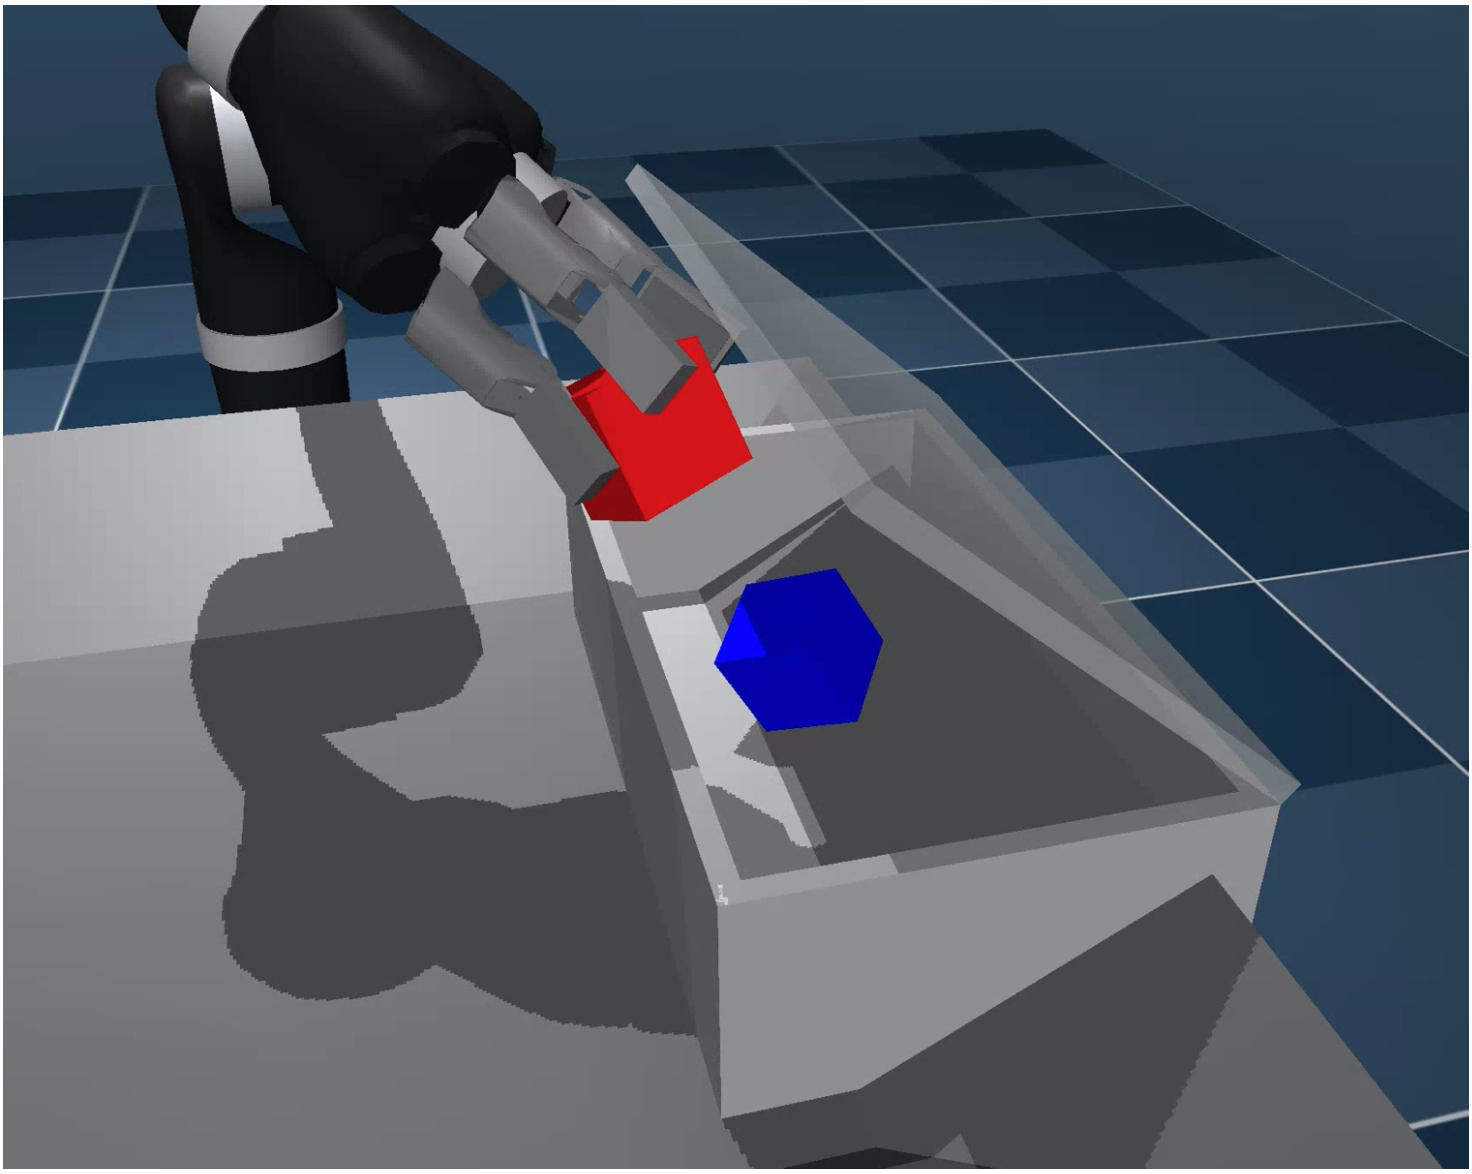
\includegraphics[scale=0.2]{sim3.png}
		
	\end{columns}
\end{frame}

\begin{frame}
	\frametitle{Experiments}
	\framesubtitle{Exp 3 - Results}
	
	\begin{figure}[!h]
		\caption{Simulation: Exp 3}
		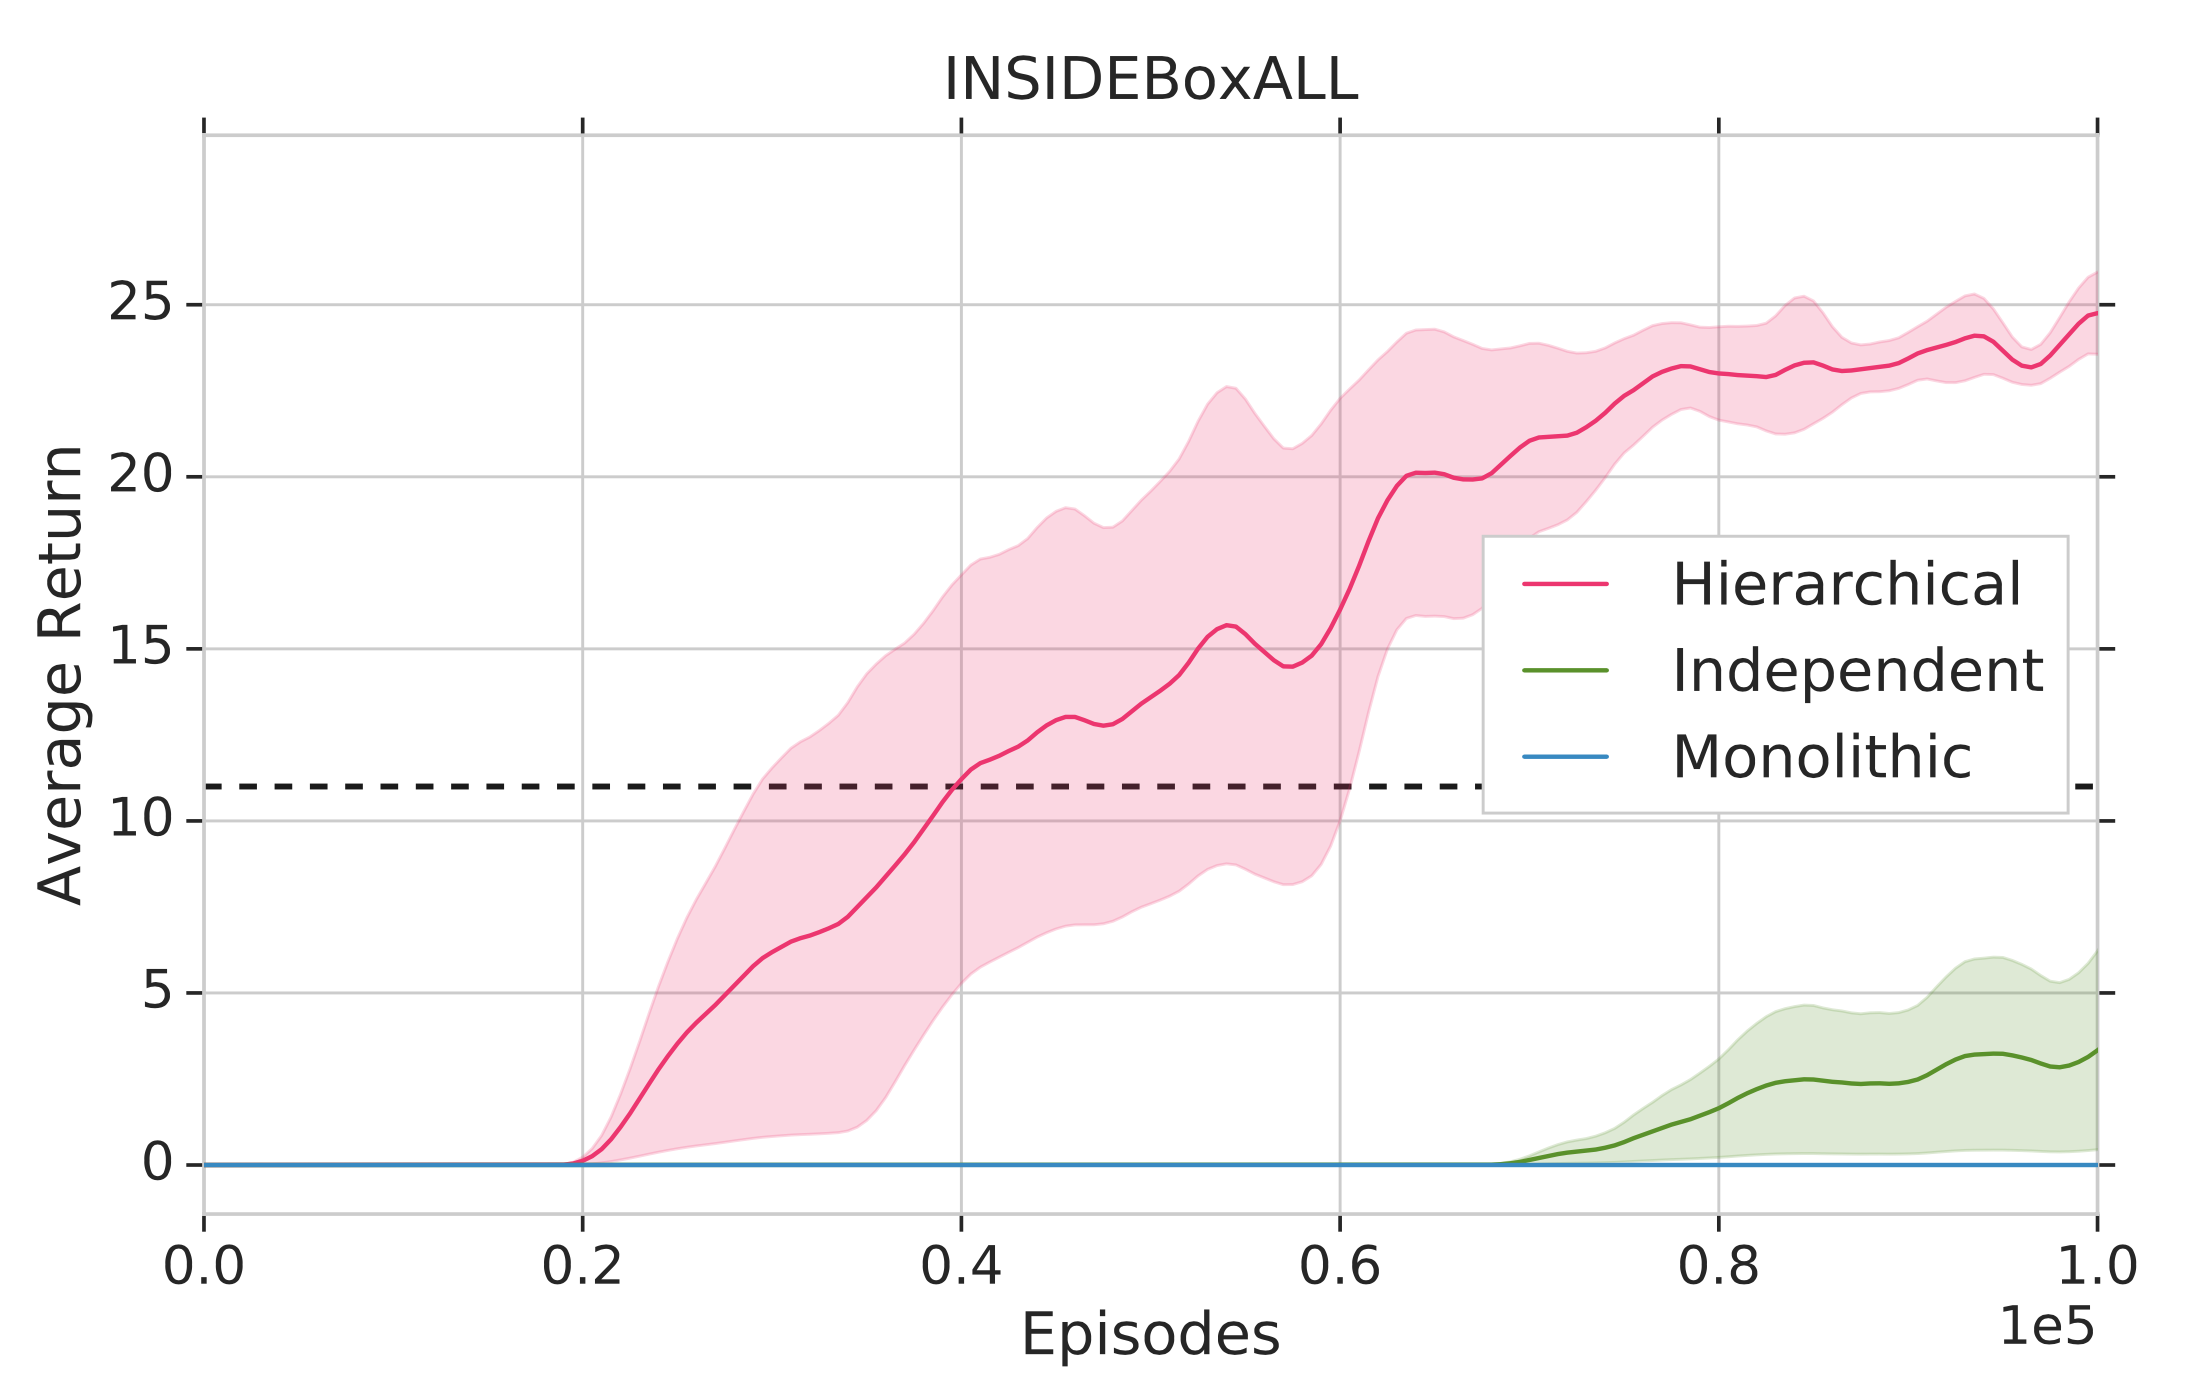
\includegraphics[scale=0.2]{sim-r3.png}
	\end{figure}
\end{frame}


\begin{frame}
	\frametitle{Conclusions and future work}
	
	\textbf{Conclusions}
	\begin{itemize}
		\item In all experiments, both on simulated and real robot, RHPO outperforms baseline models that handle tasks independently or utilize implicit sharing
		\item Sample efficiency of RHPO is much higher compared to baseline models in complex tasks
	\end{itemize}

	\textbf{Future work}
	\begin{itemize}
		\item Evaluate with direct visual input
		\item Automatic task decomposition and sub task selection
	\end{itemize}

	\nocite{abdolmaleki2018maximum} \nocite{riedmiller2018learning} \nocite{wulfmeier2019regularized}
\end{frame}

%------------------------------------------------

\begin{frame}
\frametitle{References}
\bibliography{references}
\bibliographystyle{unsrt}
\end{frame}

%------------------------------------------------

\begin{frame}
\Huge{\centerline{Thank You!}}
\end{frame}

%----------------------------------------------------------------------------------------

\end{document} 